\documentclass[twoside]{book}

% Packages required by doxygen
\usepackage{calc}
\usepackage{doxygen}
\usepackage{graphicx}
\usepackage[utf8]{inputenc}
\usepackage{makeidx}
\usepackage{multicol}
\usepackage{multirow}
\usepackage{textcomp}
\usepackage[table]{xcolor}

% NLS support packages
\usepackage[T2A]{fontenc}
\usepackage[russian]{babel}

% Font selection
\usepackage[T1]{fontenc}
\usepackage{mathptmx}
\usepackage[scaled=.90]{helvet}
\usepackage{courier}
\usepackage{amssymb}
\usepackage{sectsty}
\renewcommand{\familydefault}{\sfdefault}
\allsectionsfont{%
  \fontseries{bc}\selectfont%
  \color{darkgray}%
}
\renewcommand{\DoxyLabelFont}{%
  \fontseries{bc}\selectfont%
  \color{darkgray}%
}

% Page & text layout
\usepackage{geometry}
\geometry{%
  a4paper,%
  top=2.5cm,%
  bottom=2.5cm,%
  left=2.5cm,%
  right=2.5cm%
}
\tolerance=750
\hfuzz=15pt
\hbadness=750
\setlength{\emergencystretch}{15pt}
\setlength{\parindent}{0cm}
\setlength{\parskip}{0.2cm}
\makeatletter
\renewcommand{\paragraph}{%
  \@startsection{paragraph}{4}{0ex}{-1.0ex}{1.0ex}{%
    \normalfont\normalsize\bfseries\SS@parafont%
  }%
}
\renewcommand{\subparagraph}{%
  \@startsection{subparagraph}{5}{0ex}{-1.0ex}{1.0ex}{%
    \normalfont\normalsize\bfseries\SS@subparafont%
  }%
}
\makeatother

% Headers & footers
\usepackage{fancyhdr}
\pagestyle{fancyplain}
\fancyhead[LE]{\fancyplain{}{\bfseries\thepage}}
\fancyhead[CE]{\fancyplain{}{}}
\fancyhead[RE]{\fancyplain{}{\bfseries\leftmark}}
\fancyhead[LO]{\fancyplain{}{\bfseries\rightmark}}
\fancyhead[CO]{\fancyplain{}{}}
\fancyhead[RO]{\fancyplain{}{\bfseries\thepage}}
\fancyfoot[LE]{\fancyplain{}{}}
\fancyfoot[CE]{\fancyplain{}{}}
\fancyfoot[RE]{\fancyplain{}{\bfseries\scriptsize Документация по Radnex. Последние изменения\-: Пт 27 Май 2016 09\-:10\-:37. Создано системой Doxygen }}
\fancyfoot[LO]{\fancyplain{}{\bfseries\scriptsize Документация по Radnex. Последние изменения\-: Пт 27 Май 2016 09\-:10\-:37. Создано системой Doxygen }}
\fancyfoot[CO]{\fancyplain{}{}}
\fancyfoot[RO]{\fancyplain{}{}}
\renewcommand{\footrulewidth}{0.4pt}
\renewcommand{\chaptermark}[1]{%
  \markboth{#1}{}%
}
\renewcommand{\sectionmark}[1]{%
  \markright{\thesection\ #1}%
}

% Indices & bibliography
\usepackage{natbib}
\usepackage[titles]{tocloft}
\setcounter{tocdepth}{3}
\setcounter{secnumdepth}{5}
\makeindex

% Hyperlinks (required, but should be loaded last)
\usepackage{ifpdf}
\ifpdf
  \usepackage[pdftex,pagebackref=true]{hyperref}
\else
  \usepackage[ps2pdf,pagebackref=true]{hyperref}
\fi
\hypersetup{%
  colorlinks=true,%
  linkcolor=blue,%
  citecolor=blue,%
  unicode%
}

% Custom commands
\newcommand{\clearemptydoublepage}{%
  \newpage{\pagestyle{empty}\cleardoublepage}%
}


%===== C O N T E N T S =====

\begin{document}

% Titlepage & ToC
\hypersetup{pageanchor=false}
\pagenumbering{roman}
\begin{titlepage}
\vspace*{7cm}
\begin{center}%
{\Large Radnex }\\
\vspace*{1cm}
{\large Создано системой Doxygen 1.8.6}\\
\vspace*{0.5cm}
{\small Пт 27 Май 2016 09:10:37}\\
\end{center}
\end{titlepage}
\clearemptydoublepage
\tableofcontents
\clearemptydoublepage
\pagenumbering{arabic}
\hypersetup{pageanchor=true}

%--- Begin generated contents ---
\chapter{radnex}
\label{md_README}
\hypertarget{md_README}{}
Агрегатор соцсетей, определяющий список людей которые находятся радом 
\chapter{Иерархический список классов}
\section{Иерархия классов}
Иерархия классов.\begin{DoxyCompactList}
\item \contentsline{section}{circle}{\pageref{classcircle}}{}
\item \contentsline{section}{person}{\pageref{classperson}}{}
\begin{DoxyCompactList}
\item \contentsline{section}{admin}{\pageref{classadmin}}{}
\item \contentsline{section}{user}{\pageref{classuser}}{}
\end{DoxyCompactList}
\end{DoxyCompactList}

\chapter{Алфавитный указатель классов}
\section{Классы}
Классы с их кратким описанием.\begin{DoxyCompactList}
\item\contentsline{section}{\hyperlink{classadmin}{admin} \\*класс \char`\"{}админ\char`\"{}, пользователь, вошедший от его имени, имеет возможность просматривать информацию и удалить аккаунт любого пользователя каждом пользовател }{\pageref{classadmin}}{}
\item\contentsline{section}{\hyperlink{classcircle}{circle} \\*класс содержит информацию об окружности и методы, позволяющие изменять ее параметры }{\pageref{classcircle}}{}
\item\contentsline{section}{\hyperlink{classperson}{person} \\*базовый класс, содержит в себе общую информацию классов наследников(админ и пользователь). Не используется в программе напрямую }{\pageref{classperson}}{}
\item\contentsline{section}{\hyperlink{classuser}{user} \\*класс \char`\"{}Пользователь\char`\"{} содержит в себе всю необходимую информацию о пользователе }{\pageref{classuser}}{}
\end{DoxyCompactList}

\chapter{Список файлов}
\section{Файлы}
Полный список файлов.\begin{DoxyCompactList}
\item\contentsline{section}{\hyperlink{func_8cpp}{func.\-cpp} }{\pageref{func_8cpp}}{}
\item\contentsline{section}{\hyperlink{funkadm_8cpp}{funkadm.\-cpp} }{\pageref{funkadm_8cpp}}{}
\item\contentsline{section}{\hyperlink{main_8cpp}{main.\-cpp} }{\pageref{main_8cpp}}{}
\item\contentsline{section}{\hyperlink{main_8h}{main.\-h} }{\pageref{main_8h}}{}
\item\contentsline{section}{\hyperlink{menu_8cpp}{menu.\-cpp} }{\pageref{menu_8cpp}}{}
\item\contentsline{section}{\hyperlink{person_8h}{person.\-h} }{\pageref{person_8h}}{}
\item\contentsline{section}{\hyperlink{poisk_8cpp}{poisk.\-cpp} }{\pageref{poisk_8cpp}}{}
\end{DoxyCompactList}

\chapter{Классы}
\hypertarget{classadmin}{\section{Класс admin}
\label{classadmin}\index{admin@{admin}}
}


класс \char`\"{}админ\char`\"{}, пользователь, вошедший от его имени, имеет возможность просматривать информацию и удалить аккаунт любого пользователя каждом пользовател  




{\ttfamily \#include $<$person.\-h$>$}



Граф наследования\-:admin\-:\nopagebreak
\begin{figure}[H]
\begin{center}
\leavevmode
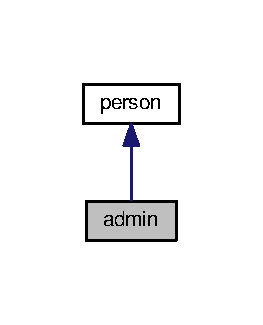
\includegraphics[width=126pt]{classadmin__inherit__graph}
\end{center}
\end{figure}


Граф связей класса admin\-:\nopagebreak
\begin{figure}[H]
\begin{center}
\leavevmode
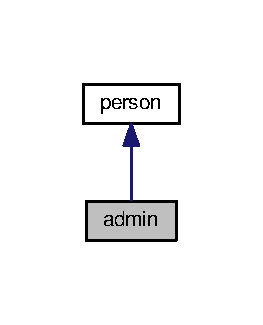
\includegraphics[width=126pt]{classadmin__coll__graph}
\end{center}
\end{figure}
\subsection*{Открытые члены}
\begin{DoxyCompactItemize}
\item 
\hyperlink{classadmin_a3460b71933fcd5a46ba70336a87f8407}{admin} ()
\begin{DoxyCompactList}\small\item\em конструктор по умолчанию \end{DoxyCompactList}\end{DoxyCompactItemize}
\subsection*{Друзья}
\begin{DoxyCompactItemize}
\item 
ostream \& \hyperlink{classadmin_ab34a42c23773278dbc4bc8802b70273d}{operator$<$$<$} (ostream \&stream, \hyperlink{classadmin}{admin} adm)
\begin{DoxyCompactList}\small\item\em перегруженй оператор $<$$<$. \end{DoxyCompactList}\item 
istream \& \hyperlink{classadmin_a68af78ea701a4eae11203e7defdc7e59}{operator$>$$>$} (istream \&stream, \hyperlink{classadmin}{admin} \&adm)
\begin{DoxyCompactList}\small\item\em перегруженый оператор $>$$>$ \end{DoxyCompactList}\end{DoxyCompactItemize}
\subsection*{Дополнительные унаследованные члены}


\subsection{Подробное описание}
класс \char`\"{}админ\char`\"{}, пользователь, вошедший от его имени, имеет возможность просматривать информацию и удалить аккаунт любого пользователя каждом пользовател 

\subsection{Конструктор(ы)}
\hypertarget{classadmin_a3460b71933fcd5a46ba70336a87f8407}{\index{admin@{admin}!admin@{admin}}
\index{admin@{admin}!admin@{admin}}
\subsubsection[{admin}]{\setlength{\rightskip}{0pt plus 5cm}admin\-::admin (
\begin{DoxyParamCaption}
{}
\end{DoxyParamCaption}
)\hspace{0.3cm}{\ttfamily [inline]}}}\label{classadmin_a3460b71933fcd5a46ba70336a87f8407}


конструктор по умолчанию 



\subsection{Документация по друзьям класса и функциям, отноносящимся к классу}
\hypertarget{classadmin_ab34a42c23773278dbc4bc8802b70273d}{\index{admin@{admin}!operator$<$$<$@{operator$<$$<$}}
\index{operator$<$$<$@{operator$<$$<$}!admin@{admin}}
\subsubsection[{operator$<$$<$}]{\setlength{\rightskip}{0pt plus 5cm}ostream\& operator$<$$<$ (
\begin{DoxyParamCaption}
\item[{ostream \&}]{stream, }
\item[{{\bf admin}}]{adm}
\end{DoxyParamCaption}
)\hspace{0.3cm}{\ttfamily [friend]}}}\label{classadmin_ab34a42c23773278dbc4bc8802b70273d}


перегруженй оператор $<$$<$. 

\hypertarget{classadmin_a68af78ea701a4eae11203e7defdc7e59}{\index{admin@{admin}!operator$>$$>$@{operator$>$$>$}}
\index{operator$>$$>$@{operator$>$$>$}!admin@{admin}}
\subsubsection[{operator$>$$>$}]{\setlength{\rightskip}{0pt plus 5cm}istream\& operator$>$$>$ (
\begin{DoxyParamCaption}
\item[{istream \&}]{stream, }
\item[{{\bf admin} \&}]{adm}
\end{DoxyParamCaption}
)\hspace{0.3cm}{\ttfamily [friend]}}}\label{classadmin_a68af78ea701a4eae11203e7defdc7e59}


перегруженый оператор $>$$>$ 



Объявления и описания членов класса находятся в файле\-:\begin{DoxyCompactItemize}
\item 
\hyperlink{person_8h}{person.\-h}\end{DoxyCompactItemize}

\hypertarget{classcircle}{\section{Класс circle}
\label{classcircle}\index{circle@{circle}}
}


класс содержит информацию об окружности и методы, позволяющие изменять ее параметры  




{\ttfamily \#include $<$person.\-h$>$}

\subsection*{Открытые члены}
\begin{DoxyCompactItemize}
\item 
\hyperlink{classcircle_a4e0786fc75051f3bbe5de2e08ef9712d}{circle} ()
\begin{DoxyCompactList}\small\item\em конструктор по умолчанию \end{DoxyCompactList}\item 
\hyperlink{classcircle_ab01e334fbdc01bad4f219ecee424795d}{circle} (unsigned int h, unsigned int i, unsigned int r)
\item 
unsigned int \hyperlink{classcircle_acb03d8b165cd8119e0db27e3d1f25973}{get\-X} () const 
\item 
unsigned int \hyperlink{classcircle_ac9a1cb1a59361d4c8aa2cfe97be9cd6b}{get\-Y} () const 
\item 
unsigned int \hyperlink{classcircle_a86f4fa52100c12e29c81a0d4cebcf47d}{get\-Rad} () const 
\item 
void \hyperlink{classcircle_a667301d843f0a0edfc92d32a43826ca7}{re\-Rad} (unsigned int r)
\item 
void \hyperlink{classcircle_a98edcf827c503e0259996abe32cb257e}{re\-Coord} (unsigned int h, unsigned int i)
\item 
void \hyperlink{classcircle_a41ac1ebe6a840fb68ea20ab9bb57be57}{showcir} () const 
\begin{DoxyCompactList}\small\item\em вывод всей информации об окружности на экран \end{DoxyCompactList}\end{DoxyCompactItemize}
\subsection*{Друзья}
\begin{DoxyCompactItemize}
\item 
ostream \& \hyperlink{classcircle_a32141087fecfdc440a1e3c16e3363dfb}{operator$<$$<$} (ostream \&stream, \hyperlink{classcircle}{circle} cir)
\begin{DoxyCompactList}\small\item\em перегруженый оператор $<$$<$. \end{DoxyCompactList}\item 
istream \& \hyperlink{classcircle_a029cd4589dbaa21d0ff2463e3a7aab52}{operator$>$$>$} (istream \&stream, \hyperlink{classcircle}{circle} \&cir)
\begin{DoxyCompactList}\small\item\em перегруженый оператор $>$$>$ \end{DoxyCompactList}\end{DoxyCompactItemize}


\subsection{Подробное описание}
класс содержит информацию об окружности и методы, позволяющие изменять ее параметры 

\subsection{Конструктор(ы)}
\hypertarget{classcircle_a4e0786fc75051f3bbe5de2e08ef9712d}{\index{circle@{circle}!circle@{circle}}
\index{circle@{circle}!circle@{circle}}
\subsubsection[{circle}]{\setlength{\rightskip}{0pt plus 5cm}circle\-::circle (
\begin{DoxyParamCaption}
{}
\end{DoxyParamCaption}
)\hspace{0.3cm}{\ttfamily [inline]}}}\label{classcircle_a4e0786fc75051f3bbe5de2e08ef9712d}


конструктор по умолчанию 

\hypertarget{classcircle_ab01e334fbdc01bad4f219ecee424795d}{\index{circle@{circle}!circle@{circle}}
\index{circle@{circle}!circle@{circle}}
\subsubsection[{circle}]{\setlength{\rightskip}{0pt plus 5cm}circle\-::circle (
\begin{DoxyParamCaption}
\item[{unsigned int}]{h, }
\item[{unsigned int}]{i, }
\item[{unsigned int}]{r}
\end{DoxyParamCaption}
)\hspace{0.3cm}{\ttfamily [inline]}}}\label{classcircle_ab01e334fbdc01bad4f219ecee424795d}
конструктор с параметрами 
\begin{DoxyParams}{Аргументы}
{\em вся} & информация об окружности \\
\hline
\end{DoxyParams}


\subsection{Методы}
\hypertarget{classcircle_a86f4fa52100c12e29c81a0d4cebcf47d}{\index{circle@{circle}!get\-Rad@{get\-Rad}}
\index{get\-Rad@{get\-Rad}!circle@{circle}}
\subsubsection[{get\-Rad}]{\setlength{\rightskip}{0pt plus 5cm}unsigned int circle\-::get\-Rad (
\begin{DoxyParamCaption}
{}
\end{DoxyParamCaption}
) const\hspace{0.3cm}{\ttfamily [inline]}}}\label{classcircle_a86f4fa52100c12e29c81a0d4cebcf47d}
\begin{DoxyReturn}{Возвращает}
rad -\/ радиус 
\end{DoxyReturn}


Граф вызова функции\-:\nopagebreak
\begin{figure}[H]
\begin{center}
\leavevmode
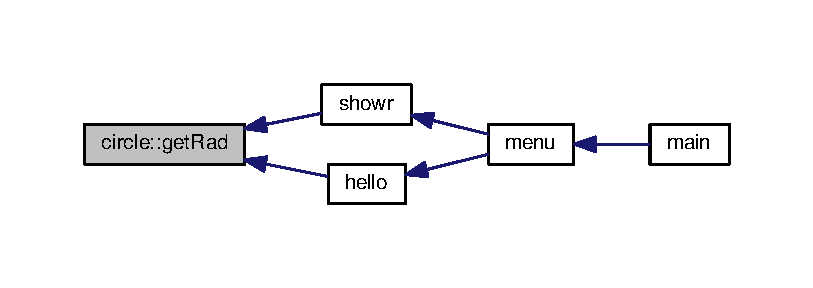
\includegraphics[width=350pt]{classcircle_a86f4fa52100c12e29c81a0d4cebcf47d_icgraph}
\end{center}
\end{figure}


\hypertarget{classcircle_acb03d8b165cd8119e0db27e3d1f25973}{\index{circle@{circle}!get\-X@{get\-X}}
\index{get\-X@{get\-X}!circle@{circle}}
\subsubsection[{get\-X}]{\setlength{\rightskip}{0pt plus 5cm}unsigned int circle\-::get\-X (
\begin{DoxyParamCaption}
{}
\end{DoxyParamCaption}
) const\hspace{0.3cm}{\ttfamily [inline]}}}\label{classcircle_acb03d8b165cd8119e0db27e3d1f25973}
\begin{DoxyReturn}{Возвращает}
х -\/ координату по Х центра окружности 
\end{DoxyReturn}


Граф вызова функции\-:\nopagebreak
\begin{figure}[H]
\begin{center}
\leavevmode
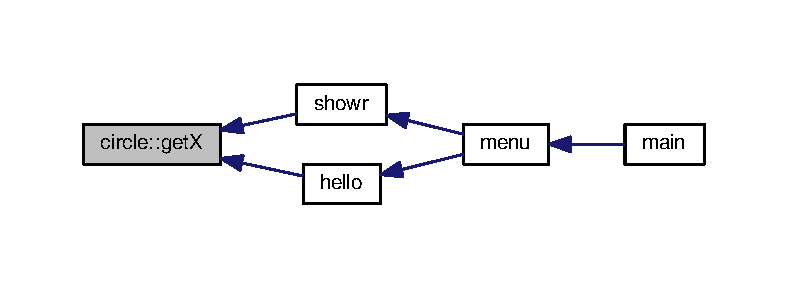
\includegraphics[width=350pt]{classcircle_acb03d8b165cd8119e0db27e3d1f25973_icgraph}
\end{center}
\end{figure}


\hypertarget{classcircle_ac9a1cb1a59361d4c8aa2cfe97be9cd6b}{\index{circle@{circle}!get\-Y@{get\-Y}}
\index{get\-Y@{get\-Y}!circle@{circle}}
\subsubsection[{get\-Y}]{\setlength{\rightskip}{0pt plus 5cm}unsigned int circle\-::get\-Y (
\begin{DoxyParamCaption}
{}
\end{DoxyParamCaption}
) const\hspace{0.3cm}{\ttfamily [inline]}}}\label{classcircle_ac9a1cb1a59361d4c8aa2cfe97be9cd6b}
\begin{DoxyReturn}{Возвращает}
y -\/ координату по у центра окружности 
\end{DoxyReturn}


Граф вызова функции\-:\nopagebreak
\begin{figure}[H]
\begin{center}
\leavevmode
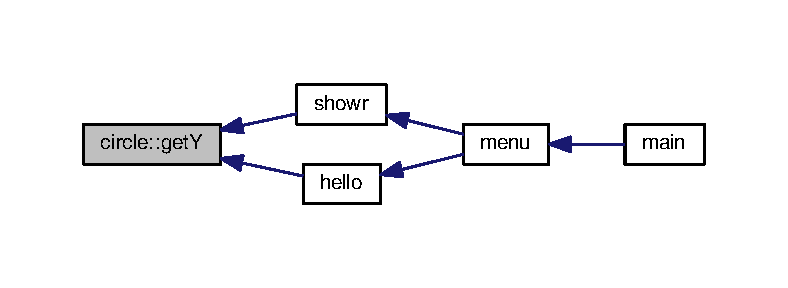
\includegraphics[width=350pt]{classcircle_ac9a1cb1a59361d4c8aa2cfe97be9cd6b_icgraph}
\end{center}
\end{figure}


\hypertarget{classcircle_a98edcf827c503e0259996abe32cb257e}{\index{circle@{circle}!re\-Coord@{re\-Coord}}
\index{re\-Coord@{re\-Coord}!circle@{circle}}
\subsubsection[{re\-Coord}]{\setlength{\rightskip}{0pt plus 5cm}void circle\-::re\-Coord (
\begin{DoxyParamCaption}
\item[{unsigned int}]{h, }
\item[{unsigned int}]{i}
\end{DoxyParamCaption}
)\hspace{0.3cm}{\ttfamily [inline]}}}\label{classcircle_a98edcf827c503e0259996abe32cb257e}
изменение координат 
\begin{DoxyParams}{Аргументы}
{\em h} & -\/ x \\
\hline
{\em i} & -\/ y \\
\hline
\end{DoxyParams}


Граф вызова функции\-:\nopagebreak
\begin{figure}[H]
\begin{center}
\leavevmode
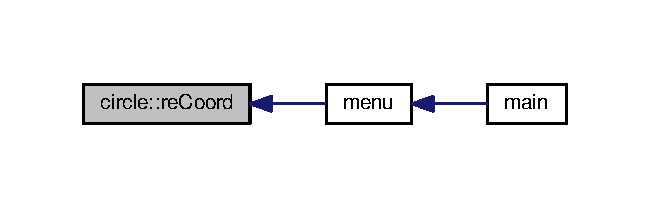
\includegraphics[width=312pt]{classcircle_a98edcf827c503e0259996abe32cb257e_icgraph}
\end{center}
\end{figure}


\hypertarget{classcircle_a667301d843f0a0edfc92d32a43826ca7}{\index{circle@{circle}!re\-Rad@{re\-Rad}}
\index{re\-Rad@{re\-Rad}!circle@{circle}}
\subsubsection[{re\-Rad}]{\setlength{\rightskip}{0pt plus 5cm}void circle\-::re\-Rad (
\begin{DoxyParamCaption}
\item[{unsigned int}]{r}
\end{DoxyParamCaption}
)\hspace{0.3cm}{\ttfamily [inline]}}}\label{classcircle_a667301d843f0a0edfc92d32a43826ca7}
изменение радиуса 
\begin{DoxyParams}{Аргументы}
{\em r} & -\/ радиус \\
\hline
\end{DoxyParams}


Граф вызова функции\-:\nopagebreak
\begin{figure}[H]
\begin{center}
\leavevmode
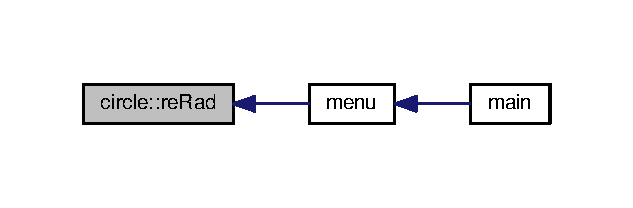
\includegraphics[width=304pt]{classcircle_a667301d843f0a0edfc92d32a43826ca7_icgraph}
\end{center}
\end{figure}


\hypertarget{classcircle_a41ac1ebe6a840fb68ea20ab9bb57be57}{\index{circle@{circle}!showcir@{showcir}}
\index{showcir@{showcir}!circle@{circle}}
\subsubsection[{showcir}]{\setlength{\rightskip}{0pt plus 5cm}void circle\-::showcir (
\begin{DoxyParamCaption}
{}
\end{DoxyParamCaption}
) const\hspace{0.3cm}{\ttfamily [inline]}}}\label{classcircle_a41ac1ebe6a840fb68ea20ab9bb57be57}


вывод всей информации об окружности на экран 



\subsection{Документация по друзьям класса и функциям, отноносящимся к классу}
\hypertarget{classcircle_a32141087fecfdc440a1e3c16e3363dfb}{\index{circle@{circle}!operator$<$$<$@{operator$<$$<$}}
\index{operator$<$$<$@{operator$<$$<$}!circle@{circle}}
\subsubsection[{operator$<$$<$}]{\setlength{\rightskip}{0pt plus 5cm}ostream\& operator$<$$<$ (
\begin{DoxyParamCaption}
\item[{ostream \&}]{stream, }
\item[{{\bf circle}}]{cir}
\end{DoxyParamCaption}
)\hspace{0.3cm}{\ttfamily [friend]}}}\label{classcircle_a32141087fecfdc440a1e3c16e3363dfb}


перегруженый оператор $<$$<$. 

\hypertarget{classcircle_a029cd4589dbaa21d0ff2463e3a7aab52}{\index{circle@{circle}!operator$>$$>$@{operator$>$$>$}}
\index{operator$>$$>$@{operator$>$$>$}!circle@{circle}}
\subsubsection[{operator$>$$>$}]{\setlength{\rightskip}{0pt plus 5cm}istream\& operator$>$$>$ (
\begin{DoxyParamCaption}
\item[{istream \&}]{stream, }
\item[{{\bf circle} \&}]{cir}
\end{DoxyParamCaption}
)\hspace{0.3cm}{\ttfamily [friend]}}}\label{classcircle_a029cd4589dbaa21d0ff2463e3a7aab52}


перегруженый оператор $>$$>$ 



Объявления и описания членов класса находятся в файле\-:\begin{DoxyCompactItemize}
\item 
\hyperlink{person_8h}{person.\-h}\end{DoxyCompactItemize}

\hypertarget{classperson}{\section{Класс person}
\label{classperson}\index{person@{person}}
}


базовый класс, содержит в себе общую информацию классов наследников(админ и пользователь). Не используется в программе напрямую  




{\ttfamily \#include $<$person.\-h$>$}



Граф наследования\-:person\-:\nopagebreak
\begin{figure}[H]
\begin{center}
\leavevmode
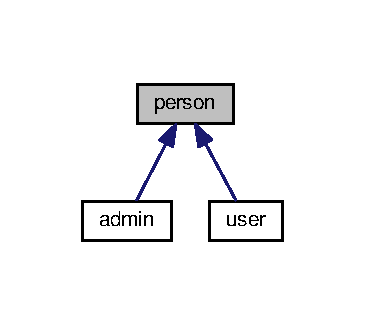
\includegraphics[width=175pt]{classperson__inherit__graph}
\end{center}
\end{figure}
\subsection*{Открытые члены}
\begin{DoxyCompactItemize}
\item 
\hyperlink{classperson_ac8851f8c7ff0e99377cf479a07333e7a}{person} ()
\begin{DoxyCompactList}\small\item\em конструктор по умолчанию \end{DoxyCompactList}\item 
\hyperlink{classperson_a3d8876846c9b757521ae56bf6a7c841a}{person} (string n, string s, string p, string m)
\item 
void \hyperlink{classperson_ab6d360263a908819b73ea80ab6fdd1c8}{re\-Pass} (string new\-P)
\item 
string \hyperlink{classperson_a76805014c07a59970b8244c79c3c6054}{get\-Sername} () const 
\item 
string \hyperlink{classperson_a8c8175284e9e52ddbf4fa3c9a04cf536}{get\-Name} () const 
\item 
string \hyperlink{classperson_a7152242a9cf64e4cc2d71ee32dbc4f4c}{get\-Mail} () const 
\item 
void \hyperlink{classperson_aa3c73bfc0527bed2c822c05d824679b0}{shov} () const 
\begin{DoxyCompactList}\small\item\em вывод на экран имени и фамилии \end{DoxyCompactList}\item 
void \hyperlink{classperson_ad27bfbd8e8c65c241abecbea2c6a0bc2}{shovad} () const 
\begin{DoxyCompactList}\small\item\em расширеный вывод информации на экран \end{DoxyCompactList}\item 
bool \hyperlink{classperson_a2ee9999b24bc3dfbc7da5003c4014d0a}{avto} (string e, string p) const 
\item 
bool \hyperlink{classperson_a120e871984ef5e815edf939331af379d}{pass} (string p) const 
\end{DoxyCompactItemize}
\subsection*{Защищенные данные}
\begin{DoxyCompactItemize}
\item 
string \hyperlink{classperson_a26e1abc114185d5c4d7d320c516d9d1e}{name}
\begin{DoxyCompactList}\small\item\em имя \end{DoxyCompactList}\item 
string \hyperlink{classperson_a8b678a1da57e030abe924a22882f6aaf}{sername}
\begin{DoxyCompactList}\small\item\em фамилия \end{DoxyCompactList}\item 
string \hyperlink{classperson_a1446508205052d36612df33f40272210}{password}
\begin{DoxyCompactList}\small\item\em пароль \end{DoxyCompactList}\item 
string \hyperlink{classperson_af68704ea11f6f084f54493b87a48200c}{mail}
\begin{DoxyCompactList}\small\item\em почта \end{DoxyCompactList}\end{DoxyCompactItemize}


\subsection{Подробное описание}
базовый класс, содержит в себе общую информацию классов наследников(админ и пользователь). Не используется в программе напрямую 

\subsection{Конструктор(ы)}
\hypertarget{classperson_ac8851f8c7ff0e99377cf479a07333e7a}{\index{person@{person}!person@{person}}
\index{person@{person}!person@{person}}
\subsubsection[{person}]{\setlength{\rightskip}{0pt plus 5cm}person\-::person (
\begin{DoxyParamCaption}
{}
\end{DoxyParamCaption}
)\hspace{0.3cm}{\ttfamily [inline]}}}\label{classperson_ac8851f8c7ff0e99377cf479a07333e7a}


конструктор по умолчанию 

\hypertarget{classperson_a3d8876846c9b757521ae56bf6a7c841a}{\index{person@{person}!person@{person}}
\index{person@{person}!person@{person}}
\subsubsection[{person}]{\setlength{\rightskip}{0pt plus 5cm}person\-::person (
\begin{DoxyParamCaption}
\item[{string}]{n, }
\item[{string}]{s, }
\item[{string}]{p, }
\item[{string}]{m}
\end{DoxyParamCaption}
)\hspace{0.3cm}{\ttfamily [inline]}}}\label{classperson_a3d8876846c9b757521ae56bf6a7c841a}
конструктор 
\begin{DoxyParams}{Аргументы}
{\em все} & параметры человека \\
\hline
\end{DoxyParams}


\subsection{Методы}
\hypertarget{classperson_a2ee9999b24bc3dfbc7da5003c4014d0a}{\index{person@{person}!avto@{avto}}
\index{avto@{avto}!person@{person}}
\subsubsection[{avto}]{\setlength{\rightskip}{0pt plus 5cm}bool person\-::avto (
\begin{DoxyParamCaption}
\item[{string}]{e, }
\item[{string}]{p}
\end{DoxyParamCaption}
) const\hspace{0.3cm}{\ttfamily [inline]}}}\label{classperson_a2ee9999b24bc3dfbc7da5003c4014d0a}
проверка на правильность введеных данных(имя, пароль) 
\begin{DoxyParams}{Аргументы}
{\em e} & -\/ почта \\
\hline
{\em p} & -\/ пароль \\
\hline
\end{DoxyParams}
\begin{DoxyReturn}{Возвращает}
true если данные совпадают, false если не совпадают 
\end{DoxyReturn}


Граф вызова функции\-:\nopagebreak
\begin{figure}[H]
\begin{center}
\leavevmode
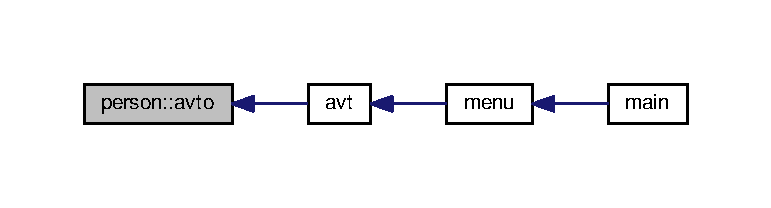
\includegraphics[width=350pt]{classperson_a2ee9999b24bc3dfbc7da5003c4014d0a_icgraph}
\end{center}
\end{figure}


\hypertarget{classperson_a7152242a9cf64e4cc2d71ee32dbc4f4c}{\index{person@{person}!get\-Mail@{get\-Mail}}
\index{get\-Mail@{get\-Mail}!person@{person}}
\subsubsection[{get\-Mail}]{\setlength{\rightskip}{0pt plus 5cm}string person\-::get\-Mail (
\begin{DoxyParamCaption}
{}
\end{DoxyParamCaption}
) const\hspace{0.3cm}{\ttfamily [inline]}}}\label{classperson_a7152242a9cf64e4cc2d71ee32dbc4f4c}
\begin{DoxyReturn}{Возвращает}
mail -\/ почту 
\end{DoxyReturn}


Граф вызова функции\-:\nopagebreak
\begin{figure}[H]
\begin{center}
\leavevmode
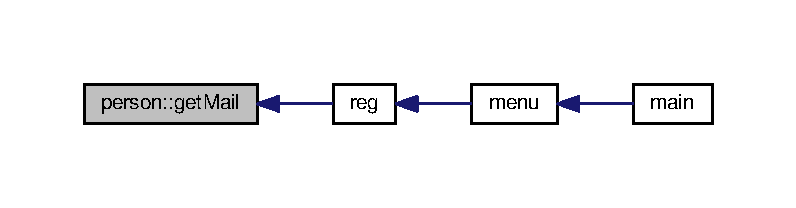
\includegraphics[width=350pt]{classperson_a7152242a9cf64e4cc2d71ee32dbc4f4c_icgraph}
\end{center}
\end{figure}


\hypertarget{classperson_a8c8175284e9e52ddbf4fa3c9a04cf536}{\index{person@{person}!get\-Name@{get\-Name}}
\index{get\-Name@{get\-Name}!person@{person}}
\subsubsection[{get\-Name}]{\setlength{\rightskip}{0pt plus 5cm}string person\-::get\-Name (
\begin{DoxyParamCaption}
{}
\end{DoxyParamCaption}
) const\hspace{0.3cm}{\ttfamily [inline]}}}\label{classperson_a8c8175284e9e52ddbf4fa3c9a04cf536}
\begin{DoxyReturn}{Возвращает}
name -\/ имя 
\end{DoxyReturn}


Граф вызова функции\-:\nopagebreak
\begin{figure}[H]
\begin{center}
\leavevmode
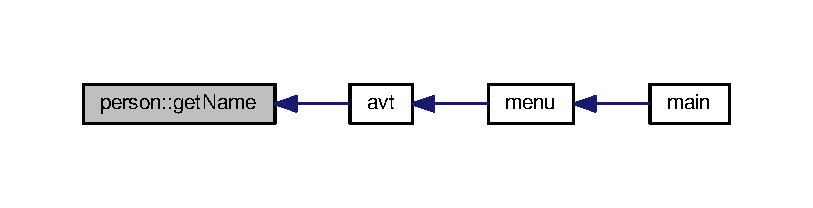
\includegraphics[width=350pt]{classperson_a8c8175284e9e52ddbf4fa3c9a04cf536_icgraph}
\end{center}
\end{figure}


\hypertarget{classperson_a76805014c07a59970b8244c79c3c6054}{\index{person@{person}!get\-Sername@{get\-Sername}}
\index{get\-Sername@{get\-Sername}!person@{person}}
\subsubsection[{get\-Sername}]{\setlength{\rightskip}{0pt plus 5cm}string person\-::get\-Sername (
\begin{DoxyParamCaption}
{}
\end{DoxyParamCaption}
) const\hspace{0.3cm}{\ttfamily [inline]}}}\label{classperson_a76805014c07a59970b8244c79c3c6054}
\begin{DoxyReturn}{Возвращает}
sername -\/ фамилию 
\end{DoxyReturn}
\hypertarget{classperson_a120e871984ef5e815edf939331af379d}{\index{person@{person}!pass@{pass}}
\index{pass@{pass}!person@{person}}
\subsubsection[{pass}]{\setlength{\rightskip}{0pt plus 5cm}bool person\-::pass (
\begin{DoxyParamCaption}
\item[{string}]{p}
\end{DoxyParamCaption}
) const\hspace{0.3cm}{\ttfamily [inline]}}}\label{classperson_a120e871984ef5e815edf939331af379d}
проверка на правильность введеного пароля 
\begin{DoxyParams}{Аргументы}
{\em p} & -\/ пароль \\
\hline
\end{DoxyParams}
\begin{DoxyReturn}{Возвращает}
true если пароль совпал, false если не совпал 
\end{DoxyReturn}


Граф вызова функции\-:\nopagebreak
\begin{figure}[H]
\begin{center}
\leavevmode
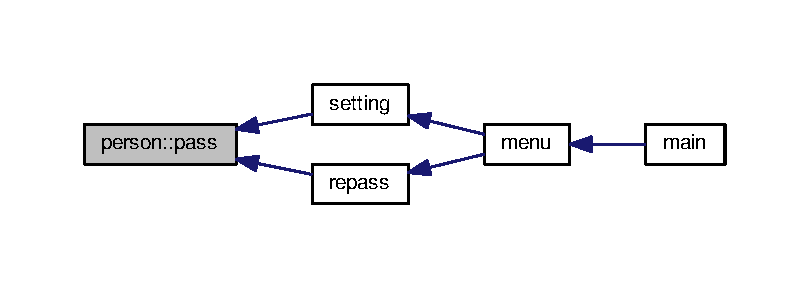
\includegraphics[width=350pt]{classperson_a120e871984ef5e815edf939331af379d_icgraph}
\end{center}
\end{figure}


\hypertarget{classperson_ab6d360263a908819b73ea80ab6fdd1c8}{\index{person@{person}!re\-Pass@{re\-Pass}}
\index{re\-Pass@{re\-Pass}!person@{person}}
\subsubsection[{re\-Pass}]{\setlength{\rightskip}{0pt plus 5cm}void person\-::re\-Pass (
\begin{DoxyParamCaption}
\item[{string}]{new\-P}
\end{DoxyParamCaption}
)\hspace{0.3cm}{\ttfamily [inline]}}}\label{classperson_ab6d360263a908819b73ea80ab6fdd1c8}
изменение пароль 
\begin{DoxyParams}{Аргументы}
{\em новый} & пароль \\
\hline
\end{DoxyParams}


Граф вызова функции\-:\nopagebreak
\begin{figure}[H]
\begin{center}
\leavevmode
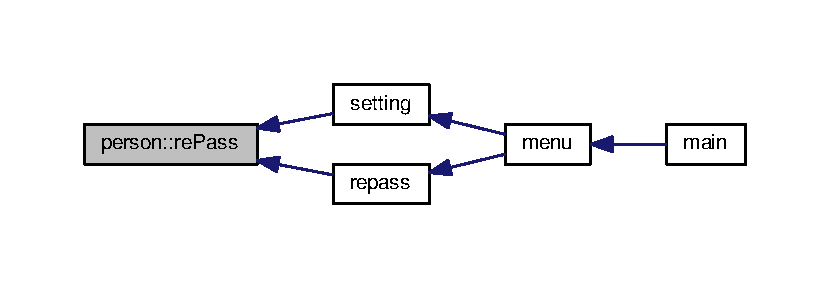
\includegraphics[width=350pt]{classperson_ab6d360263a908819b73ea80ab6fdd1c8_icgraph}
\end{center}
\end{figure}


\hypertarget{classperson_aa3c73bfc0527bed2c822c05d824679b0}{\index{person@{person}!shov@{shov}}
\index{shov@{shov}!person@{person}}
\subsubsection[{shov}]{\setlength{\rightskip}{0pt plus 5cm}void person\-::shov (
\begin{DoxyParamCaption}
{}
\end{DoxyParamCaption}
) const\hspace{0.3cm}{\ttfamily [inline]}}}\label{classperson_aa3c73bfc0527bed2c822c05d824679b0}


вывод на экран имени и фамилии 

\hypertarget{classperson_ad27bfbd8e8c65c241abecbea2c6a0bc2}{\index{person@{person}!shovad@{shovad}}
\index{shovad@{shovad}!person@{person}}
\subsubsection[{shovad}]{\setlength{\rightskip}{0pt plus 5cm}void person\-::shovad (
\begin{DoxyParamCaption}
{}
\end{DoxyParamCaption}
) const\hspace{0.3cm}{\ttfamily [inline]}}}\label{classperson_ad27bfbd8e8c65c241abecbea2c6a0bc2}


расширеный вывод информации на экран 



\subsection{Данные класса}
\hypertarget{classperson_af68704ea11f6f084f54493b87a48200c}{\index{person@{person}!mail@{mail}}
\index{mail@{mail}!person@{person}}
\subsubsection[{mail}]{\setlength{\rightskip}{0pt plus 5cm}string person\-::mail\hspace{0.3cm}{\ttfamily [protected]}}}\label{classperson_af68704ea11f6f084f54493b87a48200c}


почта 

\hypertarget{classperson_a26e1abc114185d5c4d7d320c516d9d1e}{\index{person@{person}!name@{name}}
\index{name@{name}!person@{person}}
\subsubsection[{name}]{\setlength{\rightskip}{0pt plus 5cm}string person\-::name\hspace{0.3cm}{\ttfamily [protected]}}}\label{classperson_a26e1abc114185d5c4d7d320c516d9d1e}


имя 

\hypertarget{classperson_a1446508205052d36612df33f40272210}{\index{person@{person}!password@{password}}
\index{password@{password}!person@{person}}
\subsubsection[{password}]{\setlength{\rightskip}{0pt plus 5cm}string person\-::password\hspace{0.3cm}{\ttfamily [protected]}}}\label{classperson_a1446508205052d36612df33f40272210}


пароль 

\hypertarget{classperson_a8b678a1da57e030abe924a22882f6aaf}{\index{person@{person}!sername@{sername}}
\index{sername@{sername}!person@{person}}
\subsubsection[{sername}]{\setlength{\rightskip}{0pt plus 5cm}string person\-::sername\hspace{0.3cm}{\ttfamily [protected]}}}\label{classperson_a8b678a1da57e030abe924a22882f6aaf}


фамилия 



Объявления и описания членов класса находятся в файле\-:\begin{DoxyCompactItemize}
\item 
\hyperlink{person_8h}{person.\-h}\end{DoxyCompactItemize}

\hypertarget{classuser}{\section{Класс user}
\label{classuser}\index{user@{user}}
}


класс \char`\"{}Пользователь\char`\"{} содержит в себе всю необходимую информацию о пользователе  




{\ttfamily \#include $<$person.\-h$>$}



Граф наследования\-:user\-:\nopagebreak
\begin{figure}[H]
\begin{center}
\leavevmode
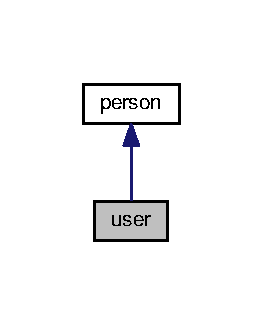
\includegraphics[width=126pt]{classuser__inherit__graph}
\end{center}
\end{figure}


Граф связей класса user\-:\nopagebreak
\begin{figure}[H]
\begin{center}
\leavevmode
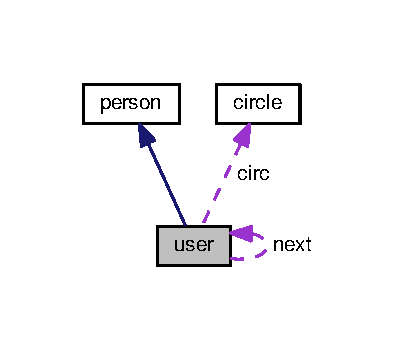
\includegraphics[width=190pt]{classuser__coll__graph}
\end{center}
\end{figure}
\subsection*{Открытые члены}
\begin{DoxyCompactItemize}
\item 
\hyperlink{classuser_a86f00bd9662cde8219dfd4601097fa3c}{user} ()
\begin{DoxyCompactList}\small\item\em конструктор по умолчанию \end{DoxyCompactList}\item 
\hyperlink{classuser_ae45f1bafa984f122d9d5eb6740f2d545}{user} (string n, string s, string p, string m, unsigned int d, unsigned int v, unsigned int i, \hyperlink{classcircle}{circle} c)
\item 
unsigned int \hyperlink{classuser_ac5da3a95d4b0afc2b4a3f007138665ba}{get\-Id} () const 
\item 
void \hyperlink{classuser_a94f7a39e4562af925d339fb62dcf6b51}{show} () const 
\begin{DoxyCompactList}\small\item\em вывод самой важной информации о пользователе \end{DoxyCompactList}\item 
void \hyperlink{classuser_ae52afec3c032697288e12b4c898f8f58}{showad} () const 
\begin{DoxyCompactList}\small\item\em расширеный вывод информации на экран \end{DoxyCompactList}\item 
void \hyperlink{classuser_a6cf4003d298be5ecb383242f4639bdb9}{hello} (const unsigned int \&id)
\item 
void \hyperlink{classuser_aedb931481b8ea24e8170923823251790}{clear\-Hi} ()
\begin{DoxyCompactList}\small\item\em очиста вектора людей, отправивших привет \end{DoxyCompactList}\end{DoxyCompactItemize}
\subsection*{Открытые атрибуты}
\begin{DoxyCompactItemize}
\item 
\hyperlink{classcircle}{circle} \hyperlink{classuser_aa3c75aaac5c22cc183ddf6da3c1a0a5e}{circ}
\item 
\hyperlink{classuser}{user} $\ast$ \hyperlink{classuser_aea47cda4229402a71223b4c5619fae97}{next}
\begin{DoxyCompactList}\small\item\em указатель на следующего пользователя \end{DoxyCompactList}\item 
vector$<$ unsigned int $>$ \hyperlink{classuser_a3818c768915004dd7263312cd5253bbd}{hi}
\end{DoxyCompactItemize}
\subsection*{Друзья}
\begin{DoxyCompactItemize}
\item 
ostream \& \hyperlink{classuser_a8dd9a408d4bec3c2e2fa99d861c3a551}{operator$<$$<$} (ostream \&stream, \hyperlink{classuser}{user} usr)
\begin{DoxyCompactList}\small\item\em перегруженый оператор $<$$<$. \end{DoxyCompactList}\item 
istream \& \hyperlink{classuser_a7fd4b22d0a1c241217d6d30c0af07078}{operator$>$$>$} (istream \&stream, \hyperlink{classuser}{user} \&usr)
\begin{DoxyCompactList}\small\item\em перегруженый оператор $>$$>$ \end{DoxyCompactList}\end{DoxyCompactItemize}
\subsection*{Дополнительные унаследованные члены}


\subsection{Подробное описание}
класс \char`\"{}Пользователь\char`\"{} содержит в себе всю необходимую информацию о пользователе 

\subsection{Конструктор(ы)}
\hypertarget{classuser_a86f00bd9662cde8219dfd4601097fa3c}{\index{user@{user}!user@{user}}
\index{user@{user}!user@{user}}
\subsubsection[{user}]{\setlength{\rightskip}{0pt plus 5cm}user\-::user (
\begin{DoxyParamCaption}
{}
\end{DoxyParamCaption}
)\hspace{0.3cm}{\ttfamily [inline]}}}\label{classuser_a86f00bd9662cde8219dfd4601097fa3c}


конструктор по умолчанию 

\hypertarget{classuser_ae45f1bafa984f122d9d5eb6740f2d545}{\index{user@{user}!user@{user}}
\index{user@{user}!user@{user}}
\subsubsection[{user}]{\setlength{\rightskip}{0pt plus 5cm}user\-::user (
\begin{DoxyParamCaption}
\item[{string}]{n, }
\item[{string}]{s, }
\item[{string}]{p, }
\item[{string}]{m, }
\item[{unsigned int}]{d, }
\item[{unsigned int}]{v, }
\item[{unsigned int}]{i, }
\item[{{\bf circle}}]{c}
\end{DoxyParamCaption}
)\hspace{0.3cm}{\ttfamily [inline]}}}\label{classuser_ae45f1bafa984f122d9d5eb6740f2d545}
конструктор с параметрами 
\begin{DoxyParams}{Аргументы}
{\em все} & параметры пользователя \\
\hline
\end{DoxyParams}


\subsection{Методы}
\hypertarget{classuser_aedb931481b8ea24e8170923823251790}{\index{user@{user}!clear\-Hi@{clear\-Hi}}
\index{clear\-Hi@{clear\-Hi}!user@{user}}
\subsubsection[{clear\-Hi}]{\setlength{\rightskip}{0pt plus 5cm}void user\-::clear\-Hi (
\begin{DoxyParamCaption}
{}
\end{DoxyParamCaption}
)\hspace{0.3cm}{\ttfamily [inline]}}}\label{classuser_aedb931481b8ea24e8170923823251790}


очиста вектора людей, отправивших привет 



Граф вызова функции\-:\nopagebreak
\begin{figure}[H]
\begin{center}
\leavevmode
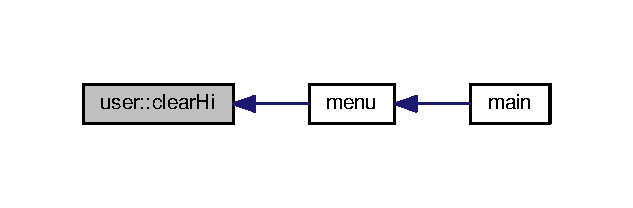
\includegraphics[width=304pt]{classuser_aedb931481b8ea24e8170923823251790_icgraph}
\end{center}
\end{figure}


\hypertarget{classuser_ac5da3a95d4b0afc2b4a3f007138665ba}{\index{user@{user}!get\-Id@{get\-Id}}
\index{get\-Id@{get\-Id}!user@{user}}
\subsubsection[{get\-Id}]{\setlength{\rightskip}{0pt plus 5cm}unsigned int user\-::get\-Id (
\begin{DoxyParamCaption}
{}
\end{DoxyParamCaption}
) const\hspace{0.3cm}{\ttfamily [inline]}}}\label{classuser_ac5da3a95d4b0afc2b4a3f007138665ba}
\begin{DoxyReturn}{Возвращает}
id -\/ id пользователя 
\end{DoxyReturn}


Граф вызова функции\-:\nopagebreak
\begin{figure}[H]
\begin{center}
\leavevmode
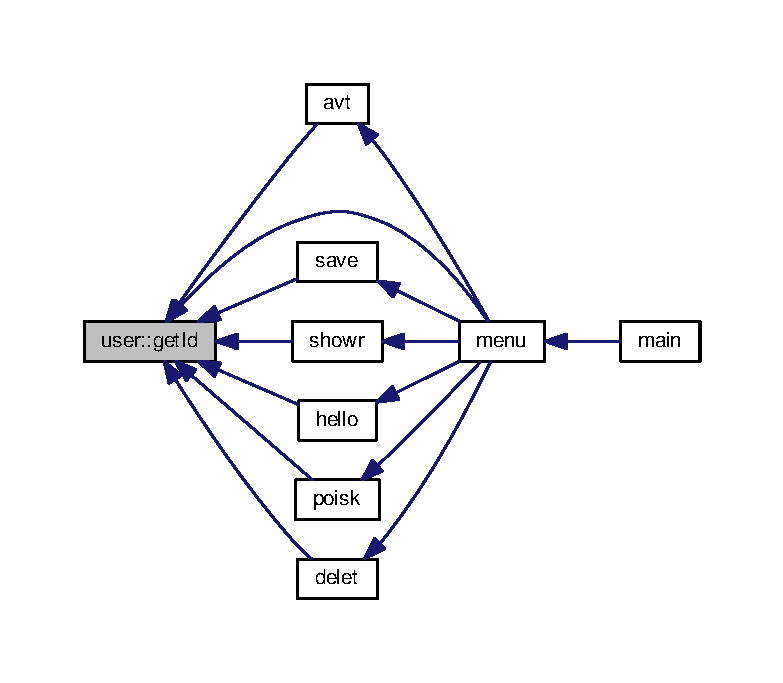
\includegraphics[width=350pt]{classuser_ac5da3a95d4b0afc2b4a3f007138665ba_icgraph}
\end{center}
\end{figure}


\hypertarget{classuser_a6cf4003d298be5ecb383242f4639bdb9}{\index{user@{user}!hello@{hello}}
\index{hello@{hello}!user@{user}}
\subsubsection[{hello}]{\setlength{\rightskip}{0pt plus 5cm}void user\-::hello (
\begin{DoxyParamCaption}
\item[{const unsigned int \&}]{id}
\end{DoxyParamCaption}
)\hspace{0.3cm}{\ttfamily [inline]}}}\label{classuser_a6cf4003d298be5ecb383242f4639bdb9}
получение привета от пользователя. функция добавляет в вектор id пользователя, отправившего \char`\"{}привет\char`\"{} 
\begin{DoxyParams}{Аргументы}
{\em id} & -\/ id пользователя, отправившего \char`\"{}привет\char`\"{} \\
\hline
\end{DoxyParams}


Граф вызова функции\-:\nopagebreak
\begin{figure}[H]
\begin{center}
\leavevmode
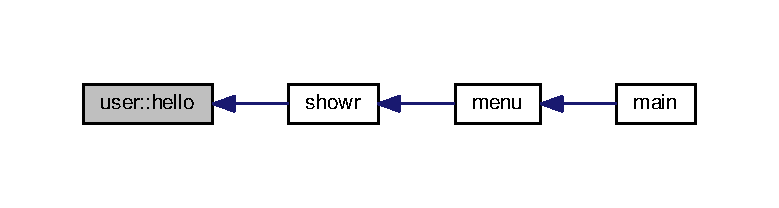
\includegraphics[width=350pt]{classuser_a6cf4003d298be5ecb383242f4639bdb9_icgraph}
\end{center}
\end{figure}


\hypertarget{classuser_a94f7a39e4562af925d339fb62dcf6b51}{\index{user@{user}!show@{show}}
\index{show@{show}!user@{user}}
\subsubsection[{show}]{\setlength{\rightskip}{0pt plus 5cm}void user\-::show (
\begin{DoxyParamCaption}
{}
\end{DoxyParamCaption}
) const\hspace{0.3cm}{\ttfamily [inline]}}}\label{classuser_a94f7a39e4562af925d339fb62dcf6b51}


вывод самой важной информации о пользователе 



Граф вызова функции\-:\nopagebreak
\begin{figure}[H]
\begin{center}
\leavevmode
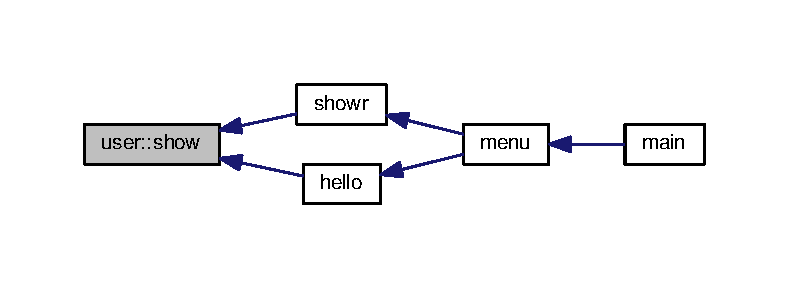
\includegraphics[width=350pt]{classuser_a94f7a39e4562af925d339fb62dcf6b51_icgraph}
\end{center}
\end{figure}


\hypertarget{classuser_ae52afec3c032697288e12b4c898f8f58}{\index{user@{user}!showad@{showad}}
\index{showad@{showad}!user@{user}}
\subsubsection[{showad}]{\setlength{\rightskip}{0pt plus 5cm}void user\-::showad (
\begin{DoxyParamCaption}
{}
\end{DoxyParamCaption}
) const\hspace{0.3cm}{\ttfamily [inline]}}}\label{classuser_ae52afec3c032697288e12b4c898f8f58}


расширеный вывод информации на экран 



Граф вызова функции\-:\nopagebreak
\begin{figure}[H]
\begin{center}
\leavevmode
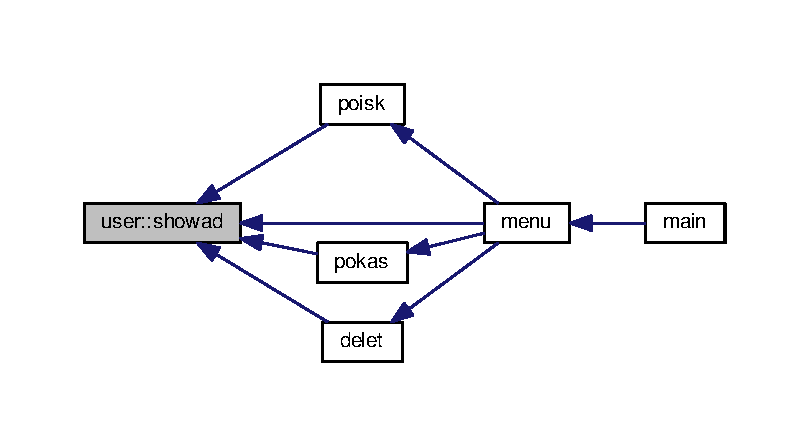
\includegraphics[width=350pt]{classuser_ae52afec3c032697288e12b4c898f8f58_icgraph}
\end{center}
\end{figure}




\subsection{Документация по друзьям класса и функциям, отноносящимся к классу}
\hypertarget{classuser_a8dd9a408d4bec3c2e2fa99d861c3a551}{\index{user@{user}!operator$<$$<$@{operator$<$$<$}}
\index{operator$<$$<$@{operator$<$$<$}!user@{user}}
\subsubsection[{operator$<$$<$}]{\setlength{\rightskip}{0pt plus 5cm}ostream\& operator$<$$<$ (
\begin{DoxyParamCaption}
\item[{ostream \&}]{stream, }
\item[{{\bf user}}]{usr}
\end{DoxyParamCaption}
)\hspace{0.3cm}{\ttfamily [friend]}}}\label{classuser_a8dd9a408d4bec3c2e2fa99d861c3a551}


перегруженый оператор $<$$<$. 

\hypertarget{classuser_a7fd4b22d0a1c241217d6d30c0af07078}{\index{user@{user}!operator$>$$>$@{operator$>$$>$}}
\index{operator$>$$>$@{operator$>$$>$}!user@{user}}
\subsubsection[{operator$>$$>$}]{\setlength{\rightskip}{0pt plus 5cm}istream\& operator$>$$>$ (
\begin{DoxyParamCaption}
\item[{istream \&}]{stream, }
\item[{{\bf user} \&}]{usr}
\end{DoxyParamCaption}
)\hspace{0.3cm}{\ttfamily [friend]}}}\label{classuser_a7fd4b22d0a1c241217d6d30c0af07078}


перегруженый оператор $>$$>$ 



\subsection{Данные класса}
\hypertarget{classuser_aa3c75aaac5c22cc183ddf6da3c1a0a5e}{\index{user@{user}!circ@{circ}}
\index{circ@{circ}!user@{user}}
\subsubsection[{circ}]{\setlength{\rightskip}{0pt plus 5cm}{\bf circle} user\-::circ}}\label{classuser_aa3c75aaac5c22cc183ddf6da3c1a0a5e}
окружность с центром в местоположении пользователя, с радиусом ,в котором он желает видеть людей \hypertarget{classuser_a3818c768915004dd7263312cd5253bbd}{\index{user@{user}!hi@{hi}}
\index{hi@{hi}!user@{user}}
\subsubsection[{hi}]{\setlength{\rightskip}{0pt plus 5cm}vector$<$unsigned int$>$ user\-::hi}}\label{classuser_a3818c768915004dd7263312cd5253bbd}
список людей отправивших \char`\"{}привет\char`\"{} \hypertarget{classuser_aea47cda4229402a71223b4c5619fae97}{\index{user@{user}!next@{next}}
\index{next@{next}!user@{user}}
\subsubsection[{next}]{\setlength{\rightskip}{0pt plus 5cm}{\bf user}$\ast$ user\-::next}}\label{classuser_aea47cda4229402a71223b4c5619fae97}


указатель на следующего пользователя 



Объявления и описания членов класса находятся в файле\-:\begin{DoxyCompactItemize}
\item 
\hyperlink{person_8h}{person.\-h}\end{DoxyCompactItemize}

\chapter{Файлы}
\hypertarget{func_8cpp}{\section{Файл func.\-cpp}
\label{func_8cpp}\index{func.\-cpp@{func.\-cpp}}
}
{\ttfamily \#include \char`\"{}main.\-h\char`\"{}}\\*
{\ttfamily \#include $<$vector$>$}\\*
{\ttfamily \#include $<$iostream$>$}\\*
{\ttfamily \#include $<$cmath$>$}\\*
{\ttfamily \#include $<$cstring$>$}\\*
{\ttfamily \#include $<$fstream$>$}\\*
Граф включаемых заголовочных файлов для func.\-cpp\-:\nopagebreak
\begin{figure}[H]
\begin{center}
\leavevmode
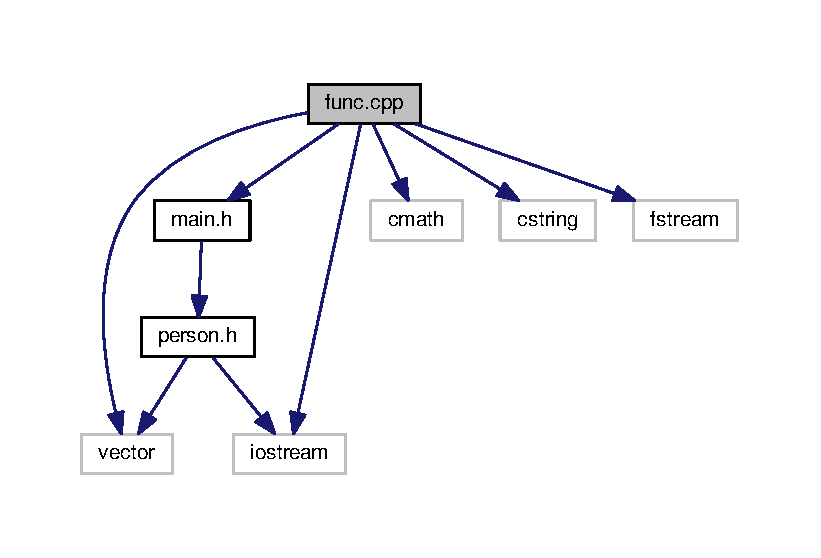
\includegraphics[width=350pt]{func_8cpp__incl}
\end{center}
\end{figure}
\subsection*{Функции}
\begin{DoxyCompactItemize}
\item 
\hyperlink{classuser}{user} $\ast$ \hyperlink{func_8cpp_a56309ab6c886ab5808deb57ee782027a}{reg} (unsigned int \&d, \hyperlink{classuser}{user} $\ast$beg, char $\ast$data)
\item 
unsigned int \hyperlink{func_8cpp_a1caa495e38a523923f4a1ddd6e9dbecc}{avt} (\hyperlink{classuser}{user} $\ast$beg, const \hyperlink{classadmin}{admin} \&adm)
\item 
ostream \& \hyperlink{func_8cpp_ab34a42c23773278dbc4bc8802b70273d}{operator$<$$<$} (ostream \&stream, \hyperlink{classadmin}{admin} adm)
\item 
istream \& \hyperlink{func_8cpp_a68af78ea701a4eae11203e7defdc7e59}{operator$>$$>$} (istream \&stream, \hyperlink{classadmin}{admin} \&adm)
\item 
ostream \& \hyperlink{func_8cpp_a8dd9a408d4bec3c2e2fa99d861c3a551}{operator$<$$<$} (ostream \&stream, \hyperlink{classuser}{user} usr)
\item 
istream \& \hyperlink{func_8cpp_a7fd4b22d0a1c241217d6d30c0af07078}{operator$>$$>$} (istream \&stream, \hyperlink{classuser}{user} \&usr)
\item 
ostream \& \hyperlink{func_8cpp_a32141087fecfdc440a1e3c16e3363dfb}{operator$<$$<$} (ostream \&stream, \hyperlink{classcircle}{circle} cir)
\item 
istream \& \hyperlink{func_8cpp_a029cd4589dbaa21d0ff2463e3a7aab52}{operator$>$$>$} (istream \&stream, \hyperlink{classcircle}{circle} \&cir)
\item 
\hyperlink{classuser}{user} $\ast$ \hyperlink{func_8cpp_ad2b7a2174e529e85e69cf24837c42bd3}{load} (char $\ast$data, \hyperlink{classadmin}{admin} \&adm)
\item 
int \hyperlink{func_8cpp_a358800d72f371bf7ef84d0d6b3873e43}{save} (char $\ast$data, \hyperlink{classuser}{user} $\ast$beg, \hyperlink{classadmin}{admin} \&adm)
\item 
bool \hyperlink{func_8cpp_ade050d1ceaa47cd21a06b898e5c89cf1}{vect} (const unsigned int \&x1, const unsigned int \&y1, const unsigned int \&x2, const unsigned int \&y2, const unsigned int \&rad)
\item 
void \hyperlink{func_8cpp_afae8672ec62ae353f834d7e0e40b6084}{showr} (\hyperlink{classuser}{user} $\ast$beg, \hyperlink{classuser}{user} $\ast$p\-U)
\item 
\hyperlink{classuser}{user} $\ast$ \hyperlink{func_8cpp_a598b17494793268fcb7d4917d3179ee2}{setting} (int \&c, \hyperlink{classuser}{user} $\ast$beg, \hyperlink{classuser}{user} $\ast$p\-U)
\item 
void \hyperlink{func_8cpp_ae49e4f4b5d423f5739a1cf8ea5f41f24}{hello} (\hyperlink{classuser}{user} $\ast$beg, \hyperlink{classuser}{user} $\ast$p\-U)
\end{DoxyCompactItemize}


\subsection{Функции}
\hypertarget{func_8cpp_a1caa495e38a523923f4a1ddd6e9dbecc}{\index{func.\-cpp@{func.\-cpp}!avt@{avt}}
\index{avt@{avt}!func.cpp@{func.\-cpp}}
\subsubsection[{avt}]{\setlength{\rightskip}{0pt plus 5cm}unsigned int avt (
\begin{DoxyParamCaption}
\item[{{\bf user} $\ast$}]{beg, }
\item[{const {\bf admin} \&}]{adm}
\end{DoxyParamCaption}
)}}\label{func_8cpp_a1caa495e38a523923f4a1ddd6e9dbecc}
функция авторизации. в зависимости от введеных почты и пароля программа может запросить ввести данные повторно, либо перейти в меню обычного пользователя, либо перейти в меню \char`\"{}адимина\char`\"{} 
\begin{DoxyParams}{Аргументы}
{\em beg} & -\/ указатель на начало списка \\
\hline
{\em adm} & -\/ объект класса \char`\"{}админ\char`\"{} \\
\hline
\end{DoxyParams}
\begin{DoxyReturn}{Возвращает}
id, авторизовавшегося пользователя 
\end{DoxyReturn}


Граф вызовов\-:\nopagebreak
\begin{figure}[H]
\begin{center}
\leavevmode
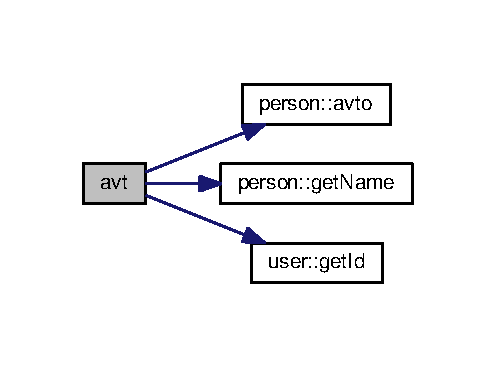
\includegraphics[width=238pt]{func_8cpp_a1caa495e38a523923f4a1ddd6e9dbecc_cgraph}
\end{center}
\end{figure}




Граф вызова функции\-:\nopagebreak
\begin{figure}[H]
\begin{center}
\leavevmode
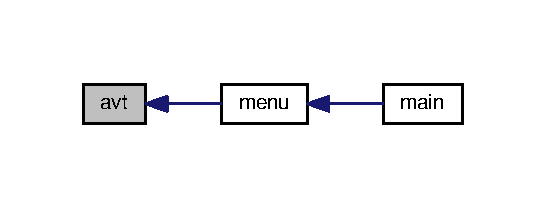
\includegraphics[width=262pt]{func_8cpp_a1caa495e38a523923f4a1ddd6e9dbecc_icgraph}
\end{center}
\end{figure}


\hypertarget{func_8cpp_ae49e4f4b5d423f5739a1cf8ea5f41f24}{\index{func.\-cpp@{func.\-cpp}!hello@{hello}}
\index{hello@{hello}!func.cpp@{func.\-cpp}}
\subsubsection[{hello}]{\setlength{\rightskip}{0pt plus 5cm}void hello (
\begin{DoxyParamCaption}
\item[{{\bf user} $\ast$}]{beg, }
\item[{{\bf user} $\ast$}]{p\-U}
\end{DoxyParamCaption}
)}}\label{func_8cpp_ae49e4f4b5d423f5739a1cf8ea5f41f24}
функция \char`\"{}привет\char`\"{} выводит на экран пользователя список людей, отправивших ему привет 
\begin{DoxyParams}{Аргументы}
{\em beg} & -\/ указатель на начало списка \\
\hline
{\em p\-U} & -\/ указатель на пользователя, на экран которого выводится список людей, отправивших ему привет \\
\hline
\end{DoxyParams}


Граф вызовов\-:\nopagebreak
\begin{figure}[H]
\begin{center}
\leavevmode
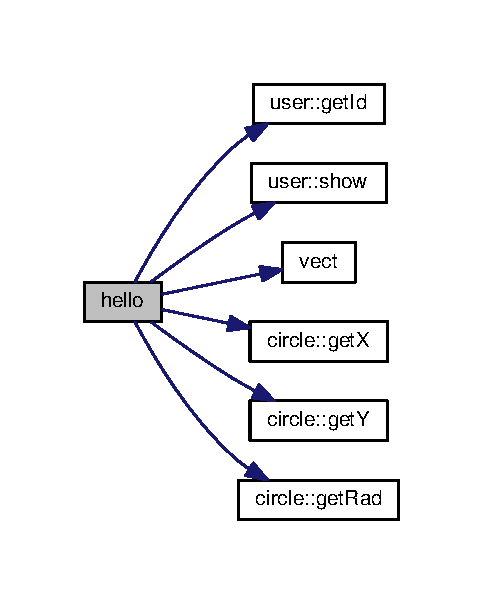
\includegraphics[width=232pt]{func_8cpp_ae49e4f4b5d423f5739a1cf8ea5f41f24_cgraph}
\end{center}
\end{figure}




Граф вызова функции\-:\nopagebreak
\begin{figure}[H]
\begin{center}
\leavevmode
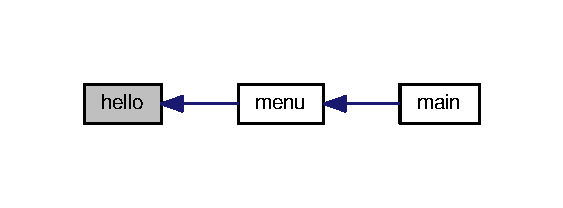
\includegraphics[width=270pt]{func_8cpp_ae49e4f4b5d423f5739a1cf8ea5f41f24_icgraph}
\end{center}
\end{figure}


\hypertarget{func_8cpp_ad2b7a2174e529e85e69cf24837c42bd3}{\index{func.\-cpp@{func.\-cpp}!load@{load}}
\index{load@{load}!func.cpp@{func.\-cpp}}
\subsubsection[{load}]{\setlength{\rightskip}{0pt plus 5cm}{\bf user}$\ast$ load (
\begin{DoxyParamCaption}
\item[{char $\ast$}]{data, }
\item[{{\bf admin} \&}]{adm}
\end{DoxyParamCaption}
)}}\label{func_8cpp_ad2b7a2174e529e85e69cf24837c42bd3}
функция загрузки списка пользователей из файла 
\begin{DoxyParams}{Аргументы}
{\em data} & -\/ название файла \\
\hline
{\em adm} & -\/ ссылка на объект класса \char`\"{}админ\char`\"{}, нужна для чтения данных админа их файла \\
\hline
\end{DoxyParams}
\begin{DoxyReturn}{Возвращает}
beg -\/ указатель на начало списка 
\end{DoxyReturn}


Граф вызова функции\-:\nopagebreak
\begin{figure}[H]
\begin{center}
\leavevmode
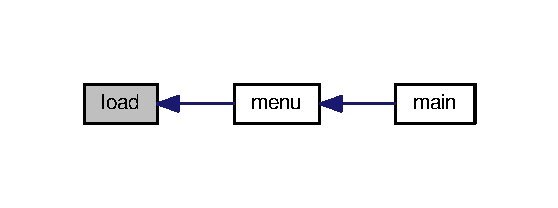
\includegraphics[width=268pt]{func_8cpp_ad2b7a2174e529e85e69cf24837c42bd3_icgraph}
\end{center}
\end{figure}


\hypertarget{func_8cpp_ab34a42c23773278dbc4bc8802b70273d}{\index{func.\-cpp@{func.\-cpp}!operator$<$$<$@{operator$<$$<$}}
\index{operator$<$$<$@{operator$<$$<$}!func.cpp@{func.\-cpp}}
\subsubsection[{operator$<$$<$}]{\setlength{\rightskip}{0pt plus 5cm}ostream\& operator$<$$<$ (
\begin{DoxyParamCaption}
\item[{ostream \&}]{stream, }
\item[{{\bf admin}}]{adm}
\end{DoxyParamCaption}
)}}\label{func_8cpp_ab34a42c23773278dbc4bc8802b70273d}
\hypertarget{func_8cpp_a8dd9a408d4bec3c2e2fa99d861c3a551}{\index{func.\-cpp@{func.\-cpp}!operator$<$$<$@{operator$<$$<$}}
\index{operator$<$$<$@{operator$<$$<$}!func.cpp@{func.\-cpp}}
\subsubsection[{operator$<$$<$}]{\setlength{\rightskip}{0pt plus 5cm}ostream\& operator$<$$<$ (
\begin{DoxyParamCaption}
\item[{ostream \&}]{stream, }
\item[{{\bf user}}]{usr}
\end{DoxyParamCaption}
)}}\label{func_8cpp_a8dd9a408d4bec3c2e2fa99d861c3a551}
\hypertarget{func_8cpp_a32141087fecfdc440a1e3c16e3363dfb}{\index{func.\-cpp@{func.\-cpp}!operator$<$$<$@{operator$<$$<$}}
\index{operator$<$$<$@{operator$<$$<$}!func.cpp@{func.\-cpp}}
\subsubsection[{operator$<$$<$}]{\setlength{\rightskip}{0pt plus 5cm}ostream\& operator$<$$<$ (
\begin{DoxyParamCaption}
\item[{ostream \&}]{stream, }
\item[{{\bf circle}}]{cir}
\end{DoxyParamCaption}
)}}\label{func_8cpp_a32141087fecfdc440a1e3c16e3363dfb}
\hypertarget{func_8cpp_a68af78ea701a4eae11203e7defdc7e59}{\index{func.\-cpp@{func.\-cpp}!operator$>$$>$@{operator$>$$>$}}
\index{operator$>$$>$@{operator$>$$>$}!func.cpp@{func.\-cpp}}
\subsubsection[{operator$>$$>$}]{\setlength{\rightskip}{0pt plus 5cm}istream\& operator$>$$>$ (
\begin{DoxyParamCaption}
\item[{istream \&}]{stream, }
\item[{{\bf admin} \&}]{adm}
\end{DoxyParamCaption}
)}}\label{func_8cpp_a68af78ea701a4eae11203e7defdc7e59}
\hypertarget{func_8cpp_a7fd4b22d0a1c241217d6d30c0af07078}{\index{func.\-cpp@{func.\-cpp}!operator$>$$>$@{operator$>$$>$}}
\index{operator$>$$>$@{operator$>$$>$}!func.cpp@{func.\-cpp}}
\subsubsection[{operator$>$$>$}]{\setlength{\rightskip}{0pt plus 5cm}istream\& operator$>$$>$ (
\begin{DoxyParamCaption}
\item[{istream \&}]{stream, }
\item[{{\bf user} \&}]{usr}
\end{DoxyParamCaption}
)}}\label{func_8cpp_a7fd4b22d0a1c241217d6d30c0af07078}
\hypertarget{func_8cpp_a029cd4589dbaa21d0ff2463e3a7aab52}{\index{func.\-cpp@{func.\-cpp}!operator$>$$>$@{operator$>$$>$}}
\index{operator$>$$>$@{operator$>$$>$}!func.cpp@{func.\-cpp}}
\subsubsection[{operator$>$$>$}]{\setlength{\rightskip}{0pt plus 5cm}istream\& operator$>$$>$ (
\begin{DoxyParamCaption}
\item[{istream \&}]{stream, }
\item[{{\bf circle} \&}]{cir}
\end{DoxyParamCaption}
)}}\label{func_8cpp_a029cd4589dbaa21d0ff2463e3a7aab52}
\hypertarget{func_8cpp_a56309ab6c886ab5808deb57ee782027a}{\index{func.\-cpp@{func.\-cpp}!reg@{reg}}
\index{reg@{reg}!func.cpp@{func.\-cpp}}
\subsubsection[{reg}]{\setlength{\rightskip}{0pt plus 5cm}{\bf user}$\ast$ reg (
\begin{DoxyParamCaption}
\item[{unsigned int \&}]{d, }
\item[{{\bf user} $\ast$}]{beg, }
\item[{char $\ast$}]{data}
\end{DoxyParamCaption}
)}}\label{func_8cpp_a56309ab6c886ab5808deb57ee782027a}
reg функция регистрации 
\begin{DoxyParams}{Аргументы}
{\em d} & -\/ id зарегистрировавшегося пользователя \\
\hline
{\em beg} & -\/ указатель на начало списка \\
\hline
{\em data} & -\/ название файла \\
\hline
\end{DoxyParams}
\begin{DoxyReturn}{Возвращает}
beg -\/ указатель на начало списка 
\end{DoxyReturn}


Граф вызовов\-:\nopagebreak
\begin{figure}[H]
\begin{center}
\leavevmode
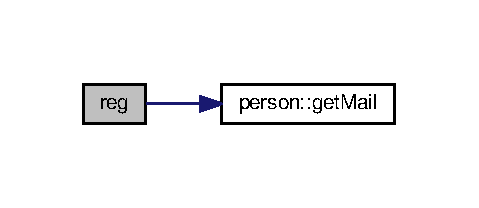
\includegraphics[width=230pt]{func_8cpp_a56309ab6c886ab5808deb57ee782027a_cgraph}
\end{center}
\end{figure}




Граф вызова функции\-:\nopagebreak
\begin{figure}[H]
\begin{center}
\leavevmode
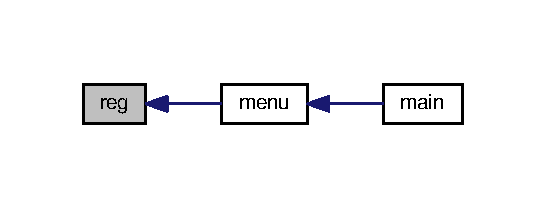
\includegraphics[width=262pt]{func_8cpp_a56309ab6c886ab5808deb57ee782027a_icgraph}
\end{center}
\end{figure}


\hypertarget{func_8cpp_a358800d72f371bf7ef84d0d6b3873e43}{\index{func.\-cpp@{func.\-cpp}!save@{save}}
\index{save@{save}!func.cpp@{func.\-cpp}}
\subsubsection[{save}]{\setlength{\rightskip}{0pt plus 5cm}int save (
\begin{DoxyParamCaption}
\item[{char $\ast$}]{data, }
\item[{{\bf user} $\ast$}]{beg, }
\item[{{\bf admin} \&}]{adm}
\end{DoxyParamCaption}
)}}\label{func_8cpp_a358800d72f371bf7ef84d0d6b3873e43}
функция сохранения списка пользователей и параметров адина в файл 
\begin{DoxyParams}{Аргументы}
{\em data} & -\/ название фйла \\
\hline
{\em beg} & -\/ указатель на начало списка \\
\hline
{\em adm} & -\/ админ \\
\hline
\end{DoxyParams}


Граф вызовов\-:\nopagebreak
\begin{figure}[H]
\begin{center}
\leavevmode
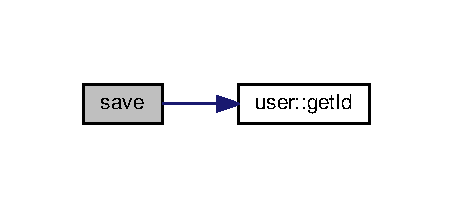
\includegraphics[width=218pt]{func_8cpp_a358800d72f371bf7ef84d0d6b3873e43_cgraph}
\end{center}
\end{figure}




Граф вызова функции\-:\nopagebreak
\begin{figure}[H]
\begin{center}
\leavevmode
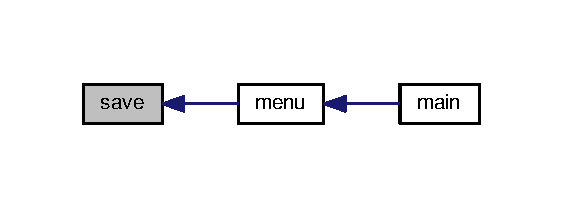
\includegraphics[width=270pt]{func_8cpp_a358800d72f371bf7ef84d0d6b3873e43_icgraph}
\end{center}
\end{figure}


\hypertarget{func_8cpp_a598b17494793268fcb7d4917d3179ee2}{\index{func.\-cpp@{func.\-cpp}!setting@{setting}}
\index{setting@{setting}!func.cpp@{func.\-cpp}}
\subsubsection[{setting}]{\setlength{\rightskip}{0pt plus 5cm}{\bf user}$\ast$ setting (
\begin{DoxyParamCaption}
\item[{int \&}]{c, }
\item[{{\bf user} $\ast$}]{beg, }
\item[{{\bf user} $\ast$}]{p\-U}
\end{DoxyParamCaption}
)}}\label{func_8cpp_a598b17494793268fcb7d4917d3179ee2}
функция -\/ меню настроек аккаунта пользователя(изменить пароль, удалить аккаунт) 
\begin{DoxyParams}{Аргументы}
{\em c} & -\/ ссылка на переменную, контролирующую дальнейший выбор пункта меню. если пользователь выбирает удаление аккаунта происходит переход в меню авторизации, в других случаях в меню пользователя \\
\hline
{\em bеg} & -\/ указатель на начало списка \\
\hline
{\em p\-U} & -\/ указатель на пользователя, который тзменяет параметры своего аккаунта \\
\hline
\end{DoxyParams}
\begin{DoxyReturn}{Возвращает}
beg -\/ указатель на начало списка 
\end{DoxyReturn}


Граф вызовов\-:\nopagebreak
\begin{figure}[H]
\begin{center}
\leavevmode
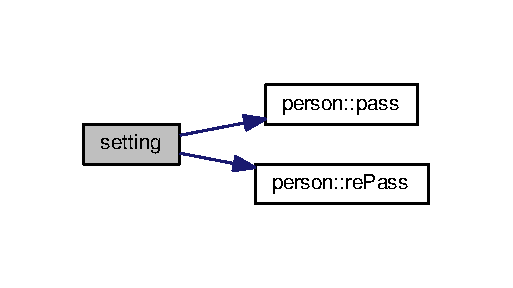
\includegraphics[width=246pt]{func_8cpp_a598b17494793268fcb7d4917d3179ee2_cgraph}
\end{center}
\end{figure}




Граф вызова функции\-:\nopagebreak
\begin{figure}[H]
\begin{center}
\leavevmode
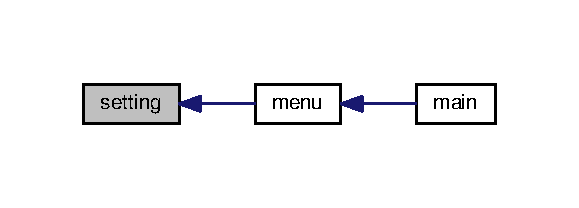
\includegraphics[width=278pt]{func_8cpp_a598b17494793268fcb7d4917d3179ee2_icgraph}
\end{center}
\end{figure}


\hypertarget{func_8cpp_afae8672ec62ae353f834d7e0e40b6084}{\index{func.\-cpp@{func.\-cpp}!showr@{showr}}
\index{showr@{showr}!func.cpp@{func.\-cpp}}
\subsubsection[{showr}]{\setlength{\rightskip}{0pt plus 5cm}void showr (
\begin{DoxyParamCaption}
\item[{{\bf user} $\ast$}]{beg, }
\item[{{\bf user} $\ast$}]{p\-U}
\end{DoxyParamCaption}
)}}\label{func_8cpp_afae8672ec62ae353f834d7e0e40b6084}
функция показа списка людей в радиусе пользователя, с информацией об их местеположении(расстояние и направление) 
\begin{DoxyParams}{Аргументы}
{\em beg} & -\/ указатель на начало списка \\
\hline
{\em p\-U} & -\/ указатель на пользователя, который ищет людей в своем радиусе \\
\hline
\end{DoxyParams}


Граф вызовов\-:\nopagebreak
\begin{figure}[H]
\begin{center}
\leavevmode
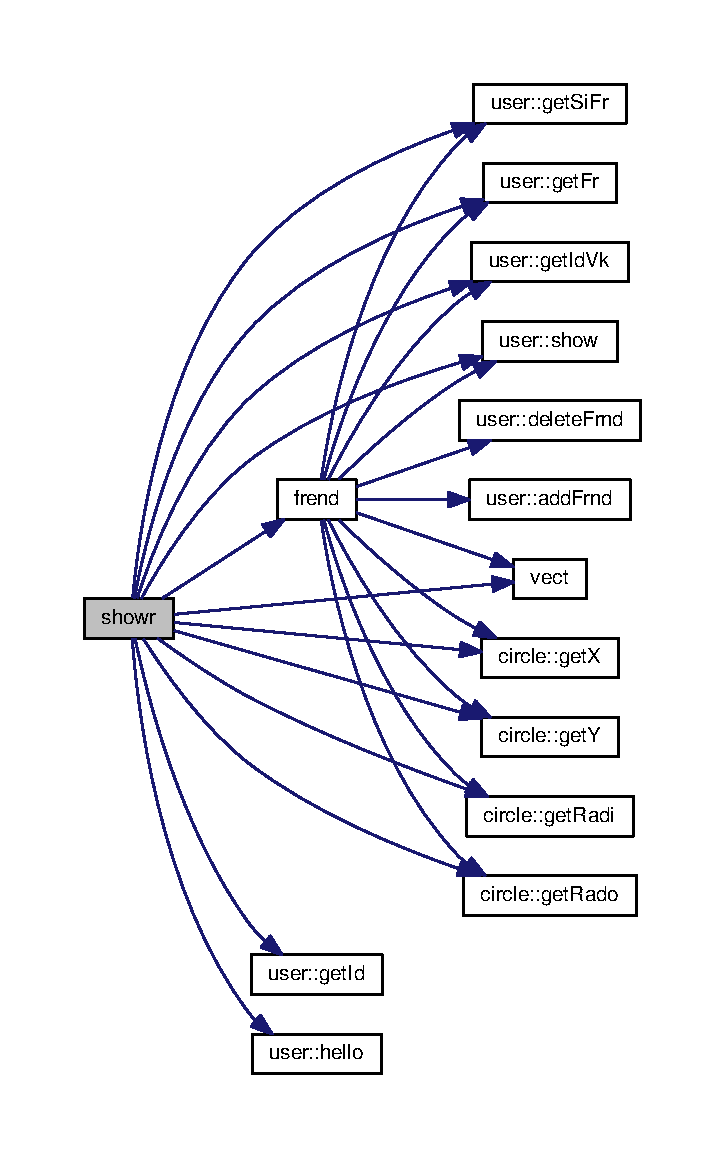
\includegraphics[width=238pt]{func_8cpp_afae8672ec62ae353f834d7e0e40b6084_cgraph}
\end{center}
\end{figure}




Граф вызова функции\-:\nopagebreak
\begin{figure}[H]
\begin{center}
\leavevmode
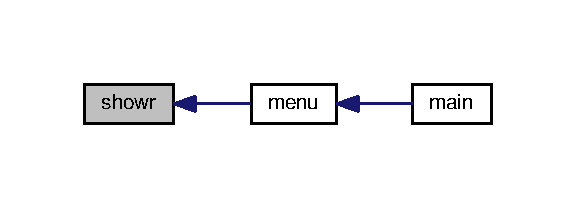
\includegraphics[width=276pt]{func_8cpp_afae8672ec62ae353f834d7e0e40b6084_icgraph}
\end{center}
\end{figure}


\hypertarget{func_8cpp_ade050d1ceaa47cd21a06b898e5c89cf1}{\index{func.\-cpp@{func.\-cpp}!vect@{vect}}
\index{vect@{vect}!func.cpp@{func.\-cpp}}
\subsubsection[{vect}]{\setlength{\rightskip}{0pt plus 5cm}bool vect (
\begin{DoxyParamCaption}
\item[{const unsigned int \&}]{x1, }
\item[{const unsigned int \&}]{y1, }
\item[{const unsigned int \&}]{x2, }
\item[{const unsigned int \&}]{y2, }
\item[{const unsigned int \&}]{rad}
\end{DoxyParamCaption}
)}}\label{func_8cpp_ade050d1ceaa47cd21a06b898e5c89cf1}
Функция показа информации о векторе в удобном для пользователя виде. Выводит на экран расстояние между точками и направление от первой точки ко второй, если расстояние между точками меньше чем радиус, в котором пользователь желает видеть людей. Имеет пять входных параметров. 
\begin{DoxyParams}{Аргументы}
{\em x1} & -\/ параметр, отвечающий за координату Х точки начала вектора \\
\hline
{\em y1} & -\/ параметр, отвечающий за координату У точки начала вектора \\
\hline
{\em x2} & -\/ параметр, отвечающий за координату Х точки конца вектора \\
\hline
{\em y2} & -\/ параметр, отвечающий за координату У точки конца вектора \\
\hline
{\em rad} & -\/ параметр, отвечающий за радиус, в котром пользователь хочет видеть дюдей \\
\hline
\end{DoxyParams}


Граф вызова функции\-:\nopagebreak
\begin{figure}[H]
\begin{center}
\leavevmode
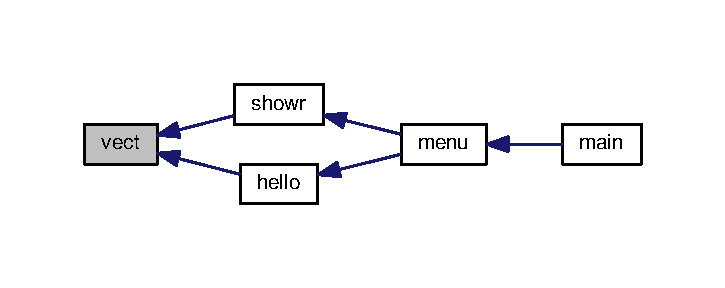
\includegraphics[width=348pt]{func_8cpp_ade050d1ceaa47cd21a06b898e5c89cf1_icgraph}
\end{center}
\end{figure}



\hypertarget{funkadm_8cpp}{\section{Файл funkadm.\-cpp}
\label{funkadm_8cpp}\index{funkadm.\-cpp@{funkadm.\-cpp}}
}
{\ttfamily \#include \char`\"{}main.\-h\char`\"{}}\\*
{\ttfamily \#include $<$iostream$>$}\\*
Граф включаемых заголовочных файлов для funkadm.\-cpp\-:\nopagebreak
\begin{figure}[H]
\begin{center}
\leavevmode
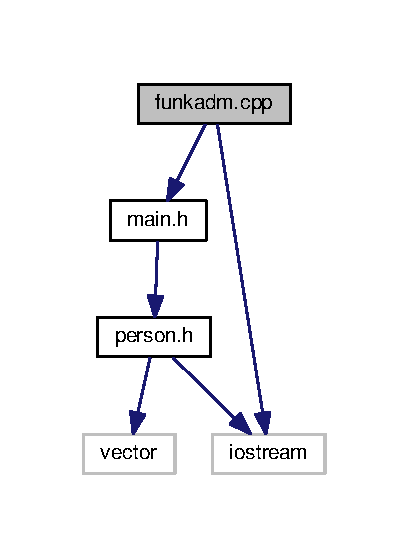
\includegraphics[width=196pt]{funkadm_8cpp__incl}
\end{center}
\end{figure}
\subsection*{Функции}
\begin{DoxyCompactItemize}
\item 
void \hyperlink{funkadm_8cpp_a8f4700d134674d7f19c2446cb6587d85}{poisk} (\hyperlink{classuser}{user} $\ast$beg)
\item 
void \hyperlink{funkadm_8cpp_ae84e6e7e36b1ecf7e591b729ad21c4de}{pokas} (\hyperlink{classuser}{user} $\ast$beg)
\item 
\hyperlink{classuser}{user} $\ast$ \hyperlink{funkadm_8cpp_a8bb3ebad2e7493f6d9b5b835c541f1fd}{delet} (\hyperlink{classuser}{user} $\ast$beg)
\item 
void \hyperlink{funkadm_8cpp_a17c795e769804ac60898af2bc625a930}{repass} (\hyperlink{classadmin}{admin} \&adm)
\end{DoxyCompactItemize}


\subsection{Функции}
\hypertarget{funkadm_8cpp_a8bb3ebad2e7493f6d9b5b835c541f1fd}{\index{funkadm.\-cpp@{funkadm.\-cpp}!delet@{delet}}
\index{delet@{delet}!funkadm.cpp@{funkadm.\-cpp}}
\subsubsection[{delet}]{\setlength{\rightskip}{0pt plus 5cm}{\bf user}$\ast$ delet (
\begin{DoxyParamCaption}
\item[{{\bf user} $\ast$}]{beg}
\end{DoxyParamCaption}
)}}\label{funkadm_8cpp_a8bb3ebad2e7493f6d9b5b835c541f1fd}
функция (админа )удаления пользователя. удаляется пользователь, выбраный админом 
\begin{DoxyParams}{Аргументы}
{\em beg-\/} & указатель на начало списка \\
\hline
\end{DoxyParams}


Граф вызовов\-:\nopagebreak
\begin{figure}[H]
\begin{center}
\leavevmode
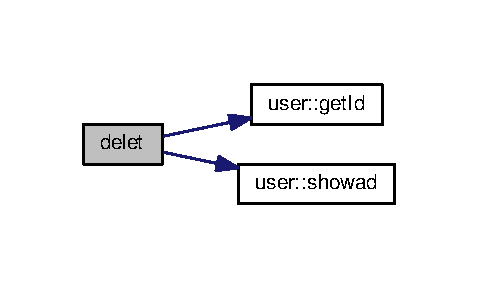
\includegraphics[width=230pt]{funkadm_8cpp_a8bb3ebad2e7493f6d9b5b835c541f1fd_cgraph}
\end{center}
\end{figure}




Граф вызова функции\-:\nopagebreak
\begin{figure}[H]
\begin{center}
\leavevmode
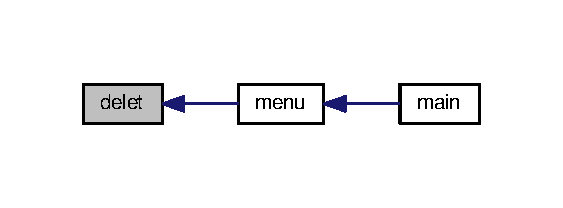
\includegraphics[width=270pt]{funkadm_8cpp_a8bb3ebad2e7493f6d9b5b835c541f1fd_icgraph}
\end{center}
\end{figure}


\hypertarget{funkadm_8cpp_a8f4700d134674d7f19c2446cb6587d85}{\index{funkadm.\-cpp@{funkadm.\-cpp}!poisk@{poisk}}
\index{poisk@{poisk}!funkadm.cpp@{funkadm.\-cpp}}
\subsubsection[{poisk}]{\setlength{\rightskip}{0pt plus 5cm}void poisk (
\begin{DoxyParamCaption}
\item[{{\bf user} $\ast$}]{beg}
\end{DoxyParamCaption}
)}}\label{funkadm_8cpp_a8f4700d134674d7f19c2446cb6587d85}
функция (админа) поиска пользователя по id. Если пользователь с введеным id существует то на экран выводится информация о нем. 
\begin{DoxyParams}{Аргументы}
{\em beg} & -\/ указатель на начало списка \\
\hline
\end{DoxyParams}


Граф вызова функции\-:\nopagebreak
\begin{figure}[H]
\begin{center}
\leavevmode
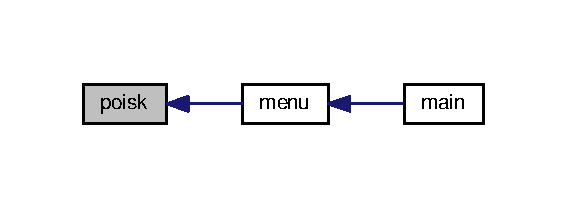
\includegraphics[width=272pt]{funkadm_8cpp_a8f4700d134674d7f19c2446cb6587d85_icgraph}
\end{center}
\end{figure}


\hypertarget{funkadm_8cpp_ae84e6e7e36b1ecf7e591b729ad21c4de}{\index{funkadm.\-cpp@{funkadm.\-cpp}!pokas@{pokas}}
\index{pokas@{pokas}!funkadm.cpp@{funkadm.\-cpp}}
\subsubsection[{pokas}]{\setlength{\rightskip}{0pt plus 5cm}void pokas (
\begin{DoxyParamCaption}
\item[{{\bf user} $\ast$}]{beg}
\end{DoxyParamCaption}
)}}\label{funkadm_8cpp_ae84e6e7e36b1ecf7e591b729ad21c4de}
функция (админа) вывода информации о каждом пользователе на экран в виде списка. 
\begin{DoxyParams}{Аргументы}
{\em beg} & -\/ указатель на начало списка \\
\hline
\end{DoxyParams}


Граф вызовов\-:\nopagebreak
\begin{figure}[H]
\begin{center}
\leavevmode
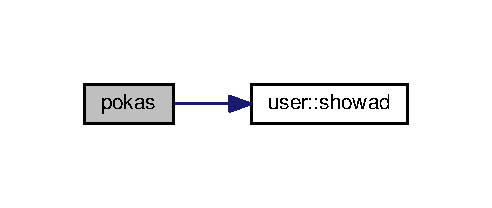
\includegraphics[width=236pt]{funkadm_8cpp_ae84e6e7e36b1ecf7e591b729ad21c4de_cgraph}
\end{center}
\end{figure}




Граф вызова функции\-:\nopagebreak
\begin{figure}[H]
\begin{center}
\leavevmode
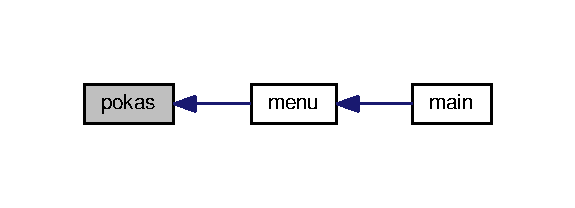
\includegraphics[width=276pt]{funkadm_8cpp_ae84e6e7e36b1ecf7e591b729ad21c4de_icgraph}
\end{center}
\end{figure}


\hypertarget{funkadm_8cpp_a17c795e769804ac60898af2bc625a930}{\index{funkadm.\-cpp@{funkadm.\-cpp}!repass@{repass}}
\index{repass@{repass}!funkadm.cpp@{funkadm.\-cpp}}
\subsubsection[{repass}]{\setlength{\rightskip}{0pt plus 5cm}void repass (
\begin{DoxyParamCaption}
\item[{{\bf admin} \&}]{adm}
\end{DoxyParamCaption}
)}}\label{funkadm_8cpp_a17c795e769804ac60898af2bc625a930}
функция (админа) изменения пароля 
\begin{DoxyParams}{Аргументы}
{\em adm} & -\/ ссылка на объект \char`\"{}админ\char`\"{} \\
\hline
\end{DoxyParams}


Граф вызовов\-:\nopagebreak
\begin{figure}[H]
\begin{center}
\leavevmode
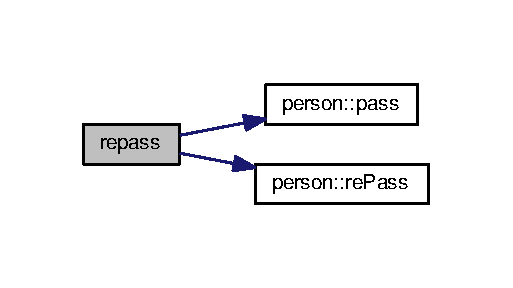
\includegraphics[width=246pt]{funkadm_8cpp_a17c795e769804ac60898af2bc625a930_cgraph}
\end{center}
\end{figure}




Граф вызова функции\-:\nopagebreak
\begin{figure}[H]
\begin{center}
\leavevmode
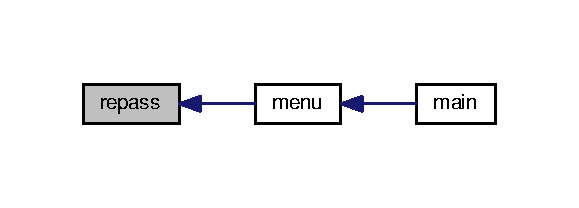
\includegraphics[width=278pt]{funkadm_8cpp_a17c795e769804ac60898af2bc625a930_icgraph}
\end{center}
\end{figure}



\hypertarget{main_8cpp}{\section{Файл main.\-cpp}
\label{main_8cpp}\index{main.\-cpp@{main.\-cpp}}
}
{\ttfamily \#include $<$iostream$>$}\\*
{\ttfamily \#include \char`\"{}main.\-h\char`\"{}}\\*
Граф включаемых заголовочных файлов для main.\-cpp\-:\nopagebreak
\begin{figure}[H]
\begin{center}
\leavevmode
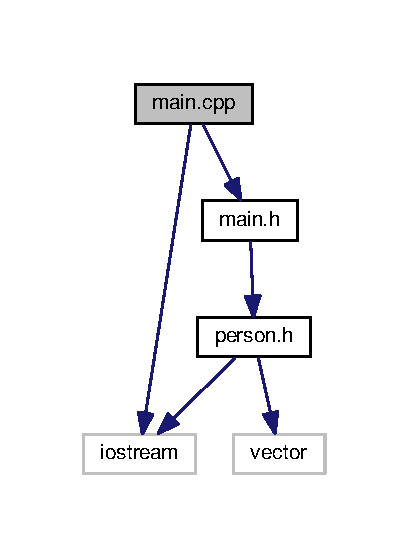
\includegraphics[width=196pt]{main_8cpp__incl}
\end{center}
\end{figure}
\subsection*{Функции}
\begin{DoxyCompactItemize}
\item 
int \hyperlink{main_8cpp_a0ddf1224851353fc92bfbff6f499fa97}{main} (int argc, char $\ast$argv\mbox{[}$\,$\mbox{]})
\end{DoxyCompactItemize}


\subsection{Функции}
\hypertarget{main_8cpp_a0ddf1224851353fc92bfbff6f499fa97}{\index{main.\-cpp@{main.\-cpp}!main@{main}}
\index{main@{main}!main.cpp@{main.\-cpp}}
\subsubsection[{main}]{\setlength{\rightskip}{0pt plus 5cm}int main (
\begin{DoxyParamCaption}
\item[{int}]{argc, }
\item[{char $\ast$}]{argv\mbox{[}$\,$\mbox{]}}
\end{DoxyParamCaption}
)}}\label{main_8cpp_a0ddf1224851353fc92bfbff6f499fa97}


Граф вызовов\-:\nopagebreak
\begin{figure}[H]
\begin{center}
\leavevmode
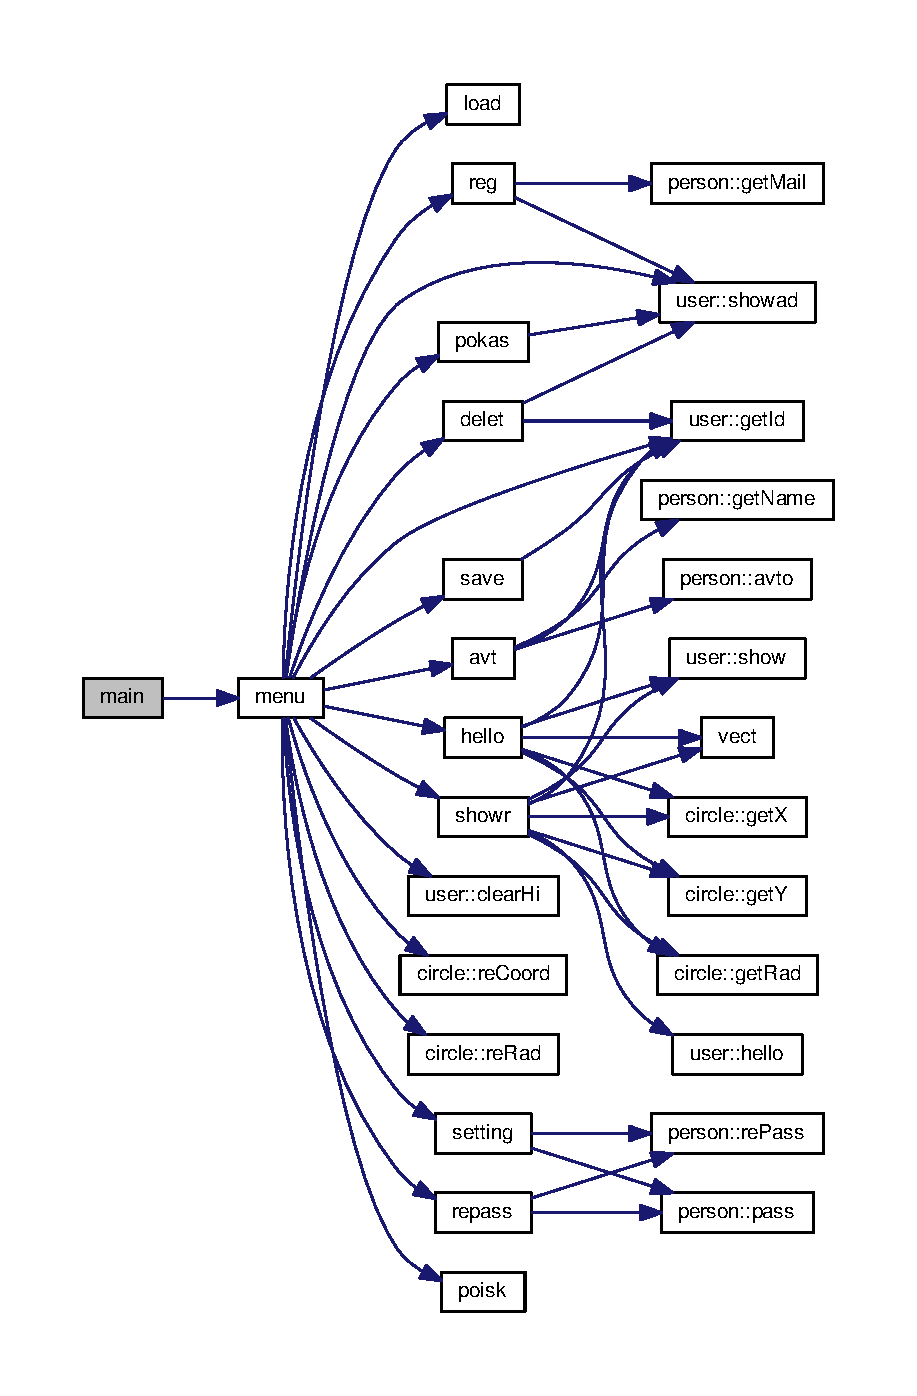
\includegraphics[width=350pt]{main_8cpp_a0ddf1224851353fc92bfbff6f499fa97_cgraph}
\end{center}
\end{figure}



\hypertarget{main_8h}{\section{Файл main.\-h}
\label{main_8h}\index{main.\-h@{main.\-h}}
}
{\ttfamily \#include \char`\"{}person.\-h\char`\"{}}\\*
Граф включаемых заголовочных файлов для main.\-h\-:\nopagebreak
\begin{figure}[H]
\begin{center}
\leavevmode
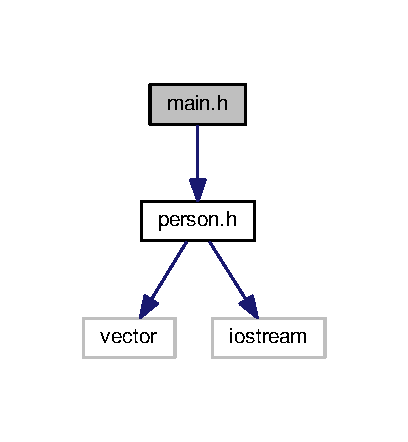
\includegraphics[width=196pt]{main_8h__incl}
\end{center}
\end{figure}
Граф файлов, в которые включается этот файл\-:
\nopagebreak
\begin{figure}[H]
\begin{center}
\leavevmode
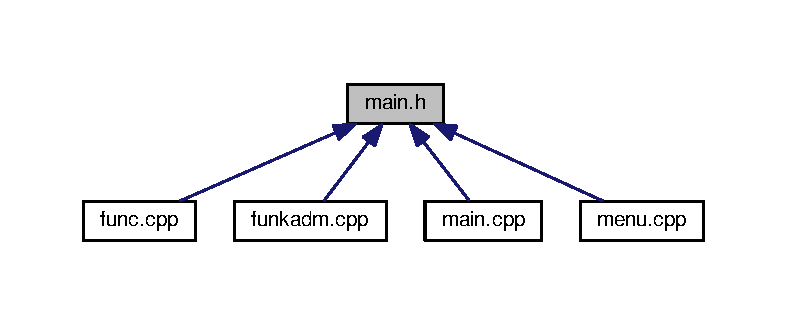
\includegraphics[width=350pt]{main_8h__dep__incl}
\end{center}
\end{figure}
\subsection*{Функции}
\begin{DoxyCompactItemize}
\item 
int \hyperlink{main_8h_a60ebaaf075977f61458d3ebe11bd44d8}{menu} (char $\ast$data)
\item 
\hyperlink{classuser}{user} $\ast$ \hyperlink{main_8h_a332687c5eb199e2bacd0b7a1bd282350}{reg} (unsigned int \&id, \hyperlink{classuser}{user} $\ast$beg, char $\ast$data)
\item 
\hyperlink{classuser}{user} $\ast$ \hyperlink{main_8h_ad2b7a2174e529e85e69cf24837c42bd3}{load} (char $\ast$data, \hyperlink{classadmin}{admin} \&adm)
\item 
int \hyperlink{main_8h_a358800d72f371bf7ef84d0d6b3873e43}{save} (char $\ast$data, \hyperlink{classuser}{user} $\ast$beg, \hyperlink{classadmin}{admin} \&adm)
\item 
unsigned int \hyperlink{main_8h_a1caa495e38a523923f4a1ddd6e9dbecc}{avt} (\hyperlink{classuser}{user} $\ast$beg, const \hyperlink{classadmin}{admin} \&adm)
\item 
void \hyperlink{main_8h_afae8672ec62ae353f834d7e0e40b6084}{showr} (\hyperlink{classuser}{user} $\ast$beg, \hyperlink{classuser}{user} $\ast$p\-U)
\item 
\hyperlink{classuser}{user} $\ast$ \hyperlink{main_8h_a598b17494793268fcb7d4917d3179ee2}{setting} (int \&c, \hyperlink{classuser}{user} $\ast$beg, \hyperlink{classuser}{user} $\ast$p\-U)
\item 
void \hyperlink{main_8h_a8f4700d134674d7f19c2446cb6587d85}{poisk} (\hyperlink{classuser}{user} $\ast$beg)
\item 
void \hyperlink{main_8h_ae84e6e7e36b1ecf7e591b729ad21c4de}{pokas} (\hyperlink{classuser}{user} $\ast$beg)
\item 
\hyperlink{classuser}{user} $\ast$ \hyperlink{main_8h_a8bb3ebad2e7493f6d9b5b835c541f1fd}{delet} (\hyperlink{classuser}{user} $\ast$beg)
\item 
void \hyperlink{main_8h_a17c795e769804ac60898af2bc625a930}{repass} (\hyperlink{classadmin}{admin} \&adm)
\item 
void \hyperlink{main_8h_ae49e4f4b5d423f5739a1cf8ea5f41f24}{hello} (\hyperlink{classuser}{user} $\ast$beg, \hyperlink{classuser}{user} $\ast$p\-U)
\item 
bool \hyperlink{main_8h_ade050d1ceaa47cd21a06b898e5c89cf1}{vect} (const unsigned int \&x1, const unsigned int \&y1, const unsigned int \&x2, const unsigned int \&y2, const unsigned int \&rad)
\item 
void \hyperlink{main_8h_ad3d705107bb5471b54db773ea8e9a3fc}{frend} (\hyperlink{classuser}{user} $\ast$beg, \hyperlink{classuser}{user} $\ast$p\-U)
\end{DoxyCompactItemize}


\subsection{Функции}
\hypertarget{main_8h_a1caa495e38a523923f4a1ddd6e9dbecc}{\index{main.\-h@{main.\-h}!avt@{avt}}
\index{avt@{avt}!main.h@{main.\-h}}
\subsubsection[{avt}]{\setlength{\rightskip}{0pt plus 5cm}unsigned int avt (
\begin{DoxyParamCaption}
\item[{{\bf user} $\ast$}]{beg, }
\item[{const {\bf admin} \&}]{adm}
\end{DoxyParamCaption}
)}}\label{main_8h_a1caa495e38a523923f4a1ddd6e9dbecc}
функция авторизации. в зависимости от введеных почты и пароля программа может запросить ввести данные повторно, либо перейти в меню обычного пользователя, либо перейти в меню \char`\"{}адимина\char`\"{} 
\begin{DoxyParams}{Аргументы}
{\em beg} & -\/ указатель на начало списка \\
\hline
{\em adm} & -\/ объект класса \char`\"{}админ\char`\"{} \\
\hline
\end{DoxyParams}
\begin{DoxyReturn}{Возвращает}
id, авторизовавшегося пользователя 
\end{DoxyReturn}


Граф вызовов\-:\nopagebreak
\begin{figure}[H]
\begin{center}
\leavevmode
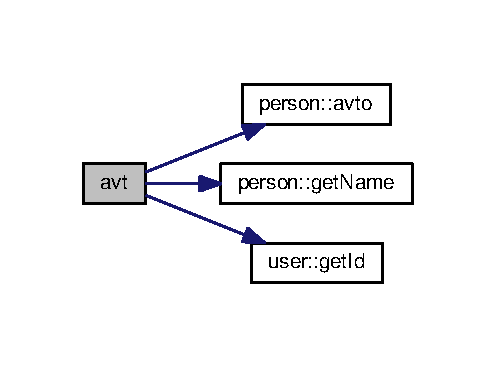
\includegraphics[width=238pt]{main_8h_a1caa495e38a523923f4a1ddd6e9dbecc_cgraph}
\end{center}
\end{figure}




Граф вызова функции\-:\nopagebreak
\begin{figure}[H]
\begin{center}
\leavevmode
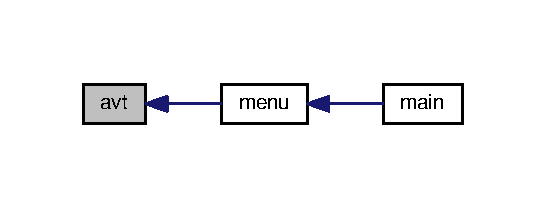
\includegraphics[width=262pt]{main_8h_a1caa495e38a523923f4a1ddd6e9dbecc_icgraph}
\end{center}
\end{figure}


\hypertarget{main_8h_a8bb3ebad2e7493f6d9b5b835c541f1fd}{\index{main.\-h@{main.\-h}!delet@{delet}}
\index{delet@{delet}!main.h@{main.\-h}}
\subsubsection[{delet}]{\setlength{\rightskip}{0pt plus 5cm}{\bf user}$\ast$ delet (
\begin{DoxyParamCaption}
\item[{{\bf user} $\ast$}]{beg}
\end{DoxyParamCaption}
)}}\label{main_8h_a8bb3ebad2e7493f6d9b5b835c541f1fd}
функция (админа )удаления пользователя. удаляется пользователь, выбраный админом 
\begin{DoxyParams}{Аргументы}
{\em beg-\/} & указатель на начало списка \\
\hline
\end{DoxyParams}


Граф вызовов\-:\nopagebreak
\begin{figure}[H]
\begin{center}
\leavevmode
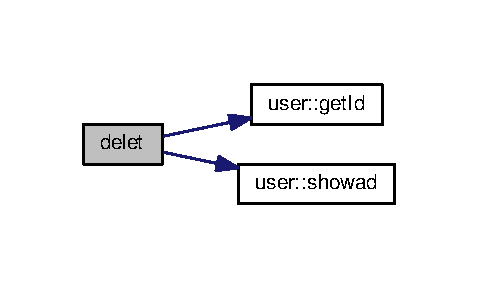
\includegraphics[width=230pt]{main_8h_a8bb3ebad2e7493f6d9b5b835c541f1fd_cgraph}
\end{center}
\end{figure}




Граф вызова функции\-:\nopagebreak
\begin{figure}[H]
\begin{center}
\leavevmode
\includegraphics[width=270pt]{main_8h_a8bb3ebad2e7493f6d9b5b835c541f1fd_icgraph}
\end{center}
\end{figure}


\hypertarget{main_8h_ad3d705107bb5471b54db773ea8e9a3fc}{\index{main.\-h@{main.\-h}!frend@{frend}}
\index{frend@{frend}!main.h@{main.\-h}}
\subsubsection[{frend}]{\setlength{\rightskip}{0pt plus 5cm}void frend (
\begin{DoxyParamCaption}
\item[{{\bf user} $\ast$}]{beg, }
\item[{{\bf user} $\ast$}]{p\-U}
\end{DoxyParamCaption}
)}}\label{main_8h_ad3d705107bb5471b54db773ea8e9a3fc}
функция -\/ меню связаное с взаимодействие пользователя со своими друзьями 
\begin{DoxyParams}{Аргументы}
{\em beg} & -\/ указатель на начало списка \\
\hline
{\em p\-U} & -\/ указатель на пользователя \\
\hline
\end{DoxyParams}
\begin{DoxyReturn}{Возвращает}
beg -\/ указатель на начало списка 
\end{DoxyReturn}


Граф вызовов\-:
\nopagebreak
\begin{figure}[H]
\begin{center}
\leavevmode
\includegraphics[width=242pt]{main_8h_ad3d705107bb5471b54db773ea8e9a3fc_cgraph}
\end{center}
\end{figure}




Граф вызова функции\-:
\nopagebreak
\begin{figure}[H]
\begin{center}
\leavevmode
\includegraphics[width=350pt]{main_8h_ad3d705107bb5471b54db773ea8e9a3fc_icgraph}
\end{center}
\end{figure}


\hypertarget{main_8h_ae49e4f4b5d423f5739a1cf8ea5f41f24}{\index{main.\-h@{main.\-h}!hello@{hello}}
\index{hello@{hello}!main.h@{main.\-h}}
\subsubsection[{hello}]{\setlength{\rightskip}{0pt plus 5cm}void hello (
\begin{DoxyParamCaption}
\item[{{\bf user} $\ast$}]{beg, }
\item[{{\bf user} $\ast$}]{p\-U}
\end{DoxyParamCaption}
)}}\label{main_8h_ae49e4f4b5d423f5739a1cf8ea5f41f24}
функция \char`\"{}привет\char`\"{} выводит на экран пользователя список людей, отправивших ему привет 
\begin{DoxyParams}{Аргументы}
{\em beg} & -\/ указатель на начало списка \\
\hline
{\em p\-U} & -\/ указатель на пользователя, на экран которого выводится список людей, отправивших ему привет \\
\hline
\end{DoxyParams}


Граф вызовов\-:
\nopagebreak
\begin{figure}[H]
\begin{center}
\leavevmode
\includegraphics[width=238pt]{main_8h_ae49e4f4b5d423f5739a1cf8ea5f41f24_cgraph}
\end{center}
\end{figure}




Граф вызова функции\-:\nopagebreak
\begin{figure}[H]
\begin{center}
\leavevmode
\includegraphics[width=270pt]{main_8h_ae49e4f4b5d423f5739a1cf8ea5f41f24_icgraph}
\end{center}
\end{figure}


\hypertarget{main_8h_ad2b7a2174e529e85e69cf24837c42bd3}{\index{main.\-h@{main.\-h}!load@{load}}
\index{load@{load}!main.h@{main.\-h}}
\subsubsection[{load}]{\setlength{\rightskip}{0pt plus 5cm}{\bf user}$\ast$ load (
\begin{DoxyParamCaption}
\item[{char $\ast$}]{data, }
\item[{{\bf admin} \&}]{adm}
\end{DoxyParamCaption}
)}}\label{main_8h_ad2b7a2174e529e85e69cf24837c42bd3}
функция загрузки списка пользователей из файла 
\begin{DoxyParams}{Аргументы}
{\em data} & -\/ название файла \\
\hline
{\em adm} & -\/ ссылка на объект класса \char`\"{}админ\char`\"{}, нужна для чтения данных админа их файла \\
\hline
\end{DoxyParams}
\begin{DoxyReturn}{Возвращает}
beg -\/ указатель на начало списка 
\end{DoxyReturn}


Граф вызова функции\-:\nopagebreak
\begin{figure}[H]
\begin{center}
\leavevmode
\includegraphics[width=268pt]{main_8h_ad2b7a2174e529e85e69cf24837c42bd3_icgraph}
\end{center}
\end{figure}


\hypertarget{main_8h_a60ebaaf075977f61458d3ebe11bd44d8}{\index{main.\-h@{main.\-h}!menu@{menu}}
\index{menu@{menu}!main.h@{main.\-h}}
\subsubsection[{menu}]{\setlength{\rightskip}{0pt plus 5cm}int menu (
\begin{DoxyParamCaption}
\item[{char $\ast$}]{data}
\end{DoxyParamCaption}
)}}\label{main_8h_a60ebaaf075977f61458d3ebe11bd44d8}
меню 
\begin{DoxyParams}{Аргументы}
{\em data} & -\/ имя файла со всей информацией о пользователях \\
\hline
\end{DoxyParams}


Граф вызовов\-:
\nopagebreak
\begin{figure}[H]
\begin{center}
\leavevmode
\includegraphics[height=550pt]{main_8h_a60ebaaf075977f61458d3ebe11bd44d8_cgraph}
\end{center}
\end{figure}




Граф вызова функции\-:\nopagebreak
\begin{figure}[H]
\begin{center}
\leavevmode
\includegraphics[width=196pt]{main_8h_a60ebaaf075977f61458d3ebe11bd44d8_icgraph}
\end{center}
\end{figure}


\hypertarget{main_8h_a8f4700d134674d7f19c2446cb6587d85}{\index{main.\-h@{main.\-h}!poisk@{poisk}}
\index{poisk@{poisk}!main.h@{main.\-h}}
\subsubsection[{poisk}]{\setlength{\rightskip}{0pt plus 5cm}void poisk (
\begin{DoxyParamCaption}
\item[{{\bf user} $\ast$}]{beg}
\end{DoxyParamCaption}
)}}\label{main_8h_a8f4700d134674d7f19c2446cb6587d85}
функция (админа) поиска пользователя по id. Если пользователь с введеным id существует то на экран выводится информация о нем. 
\begin{DoxyParams}{Аргументы}
{\em beg} & -\/ указатель на начало списка \\
\hline
\end{DoxyParams}


Граф вызовов\-:\nopagebreak
\begin{figure}[H]
\begin{center}
\leavevmode
\includegraphics[width=232pt]{main_8h_a8f4700d134674d7f19c2446cb6587d85_cgraph}
\end{center}
\end{figure}




Граф вызова функции\-:\nopagebreak
\begin{figure}[H]
\begin{center}
\leavevmode
\includegraphics[width=272pt]{main_8h_a8f4700d134674d7f19c2446cb6587d85_icgraph}
\end{center}
\end{figure}


\hypertarget{main_8h_ae84e6e7e36b1ecf7e591b729ad21c4de}{\index{main.\-h@{main.\-h}!pokas@{pokas}}
\index{pokas@{pokas}!main.h@{main.\-h}}
\subsubsection[{pokas}]{\setlength{\rightskip}{0pt plus 5cm}void pokas (
\begin{DoxyParamCaption}
\item[{{\bf user} $\ast$}]{beg}
\end{DoxyParamCaption}
)}}\label{main_8h_ae84e6e7e36b1ecf7e591b729ad21c4de}
функция (админа) вывода информации о каждом пользователе на экран в виде списка. 
\begin{DoxyParams}{Аргументы}
{\em beg} & -\/ указатель на начало списка \\
\hline
\end{DoxyParams}


Граф вызовов\-:\nopagebreak
\begin{figure}[H]
\begin{center}
\leavevmode
\includegraphics[width=236pt]{main_8h_ae84e6e7e36b1ecf7e591b729ad21c4de_cgraph}
\end{center}
\end{figure}




Граф вызова функции\-:\nopagebreak
\begin{figure}[H]
\begin{center}
\leavevmode
\includegraphics[width=276pt]{main_8h_ae84e6e7e36b1ecf7e591b729ad21c4de_icgraph}
\end{center}
\end{figure}


\hypertarget{main_8h_a332687c5eb199e2bacd0b7a1bd282350}{\index{main.\-h@{main.\-h}!reg@{reg}}
\index{reg@{reg}!main.h@{main.\-h}}
\subsubsection[{reg}]{\setlength{\rightskip}{0pt plus 5cm}{\bf user}$\ast$ reg (
\begin{DoxyParamCaption}
\item[{unsigned int \&}]{d, }
\item[{{\bf user} $\ast$}]{beg, }
\item[{char $\ast$}]{data}
\end{DoxyParamCaption}
)}}\label{main_8h_a332687c5eb199e2bacd0b7a1bd282350}
reg функция регистрации 
\begin{DoxyParams}{Аргументы}
{\em d} & -\/ id зарегистрировавшегося пользователя \\
\hline
{\em beg} & -\/ указатель на начало списка \\
\hline
{\em data} & -\/ название файла \\
\hline
\end{DoxyParams}
\begin{DoxyReturn}{Возвращает}
beg -\/ указатель на начало списка 
\end{DoxyReturn}


Граф вызовов\-:
\nopagebreak
\begin{figure}[H]
\begin{center}
\leavevmode
\includegraphics[width=230pt]{main_8h_a332687c5eb199e2bacd0b7a1bd282350_cgraph}
\end{center}
\end{figure}




Граф вызова функции\-:\nopagebreak
\begin{figure}[H]
\begin{center}
\leavevmode
\includegraphics[width=262pt]{main_8h_a332687c5eb199e2bacd0b7a1bd282350_icgraph}
\end{center}
\end{figure}


\hypertarget{main_8h_a17c795e769804ac60898af2bc625a930}{\index{main.\-h@{main.\-h}!repass@{repass}}
\index{repass@{repass}!main.h@{main.\-h}}
\subsubsection[{repass}]{\setlength{\rightskip}{0pt plus 5cm}void repass (
\begin{DoxyParamCaption}
\item[{{\bf admin} \&}]{adm}
\end{DoxyParamCaption}
)}}\label{main_8h_a17c795e769804ac60898af2bc625a930}
функция (админа) изменения пароля 
\begin{DoxyParams}{Аргументы}
{\em adm} & -\/ ссылка на объект \char`\"{}админ\char`\"{} \\
\hline
\end{DoxyParams}


Граф вызовов\-:\nopagebreak
\begin{figure}[H]
\begin{center}
\leavevmode
\includegraphics[width=246pt]{main_8h_a17c795e769804ac60898af2bc625a930_cgraph}
\end{center}
\end{figure}




Граф вызова функции\-:\nopagebreak
\begin{figure}[H]
\begin{center}
\leavevmode
\includegraphics[width=278pt]{main_8h_a17c795e769804ac60898af2bc625a930_icgraph}
\end{center}
\end{figure}


\hypertarget{main_8h_a358800d72f371bf7ef84d0d6b3873e43}{\index{main.\-h@{main.\-h}!save@{save}}
\index{save@{save}!main.h@{main.\-h}}
\subsubsection[{save}]{\setlength{\rightskip}{0pt plus 5cm}int save (
\begin{DoxyParamCaption}
\item[{char $\ast$}]{data, }
\item[{{\bf user} $\ast$}]{beg, }
\item[{{\bf admin} \&}]{adm}
\end{DoxyParamCaption}
)}}\label{main_8h_a358800d72f371bf7ef84d0d6b3873e43}
функция сохранения списка пользователей и параметров адина в файл 
\begin{DoxyParams}{Аргументы}
{\em data} & -\/ название фйла \\
\hline
{\em beg} & -\/ указатель на начало списка \\
\hline
{\em adm} & -\/ админ \\
\hline
\end{DoxyParams}


Граф вызовов\-:\nopagebreak
\begin{figure}[H]
\begin{center}
\leavevmode
\includegraphics[width=218pt]{main_8h_a358800d72f371bf7ef84d0d6b3873e43_cgraph}
\end{center}
\end{figure}




Граф вызова функции\-:\nopagebreak
\begin{figure}[H]
\begin{center}
\leavevmode
\includegraphics[width=270pt]{main_8h_a358800d72f371bf7ef84d0d6b3873e43_icgraph}
\end{center}
\end{figure}


\hypertarget{main_8h_a598b17494793268fcb7d4917d3179ee2}{\index{main.\-h@{main.\-h}!setting@{setting}}
\index{setting@{setting}!main.h@{main.\-h}}
\subsubsection[{setting}]{\setlength{\rightskip}{0pt plus 5cm}{\bf user}$\ast$ setting (
\begin{DoxyParamCaption}
\item[{int \&}]{c, }
\item[{{\bf user} $\ast$}]{beg, }
\item[{{\bf user} $\ast$}]{p\-U}
\end{DoxyParamCaption}
)}}\label{main_8h_a598b17494793268fcb7d4917d3179ee2}
функция -\/ меню настроек аккаунта пользователя(изменить пароль, удалить аккаунт) 
\begin{DoxyParams}{Аргументы}
{\em c} & -\/ ссылка на переменную, контролирующую дальнейший выбор пункта меню. если пользователь выбирает удаление аккаунта происходит переход в меню авторизации, в других случаях в меню пользователя \\
\hline
{\em bеg} & -\/ указатель на начало списка \\
\hline
{\em p\-U} & -\/ указатель на пользователя, который тзменяет параметры своего аккаунта \\
\hline
\end{DoxyParams}
\begin{DoxyReturn}{Возвращает}
beg -\/ указатель на начало списка 
\end{DoxyReturn}


Граф вызовов\-:\nopagebreak
\begin{figure}[H]
\begin{center}
\leavevmode
\includegraphics[width=246pt]{main_8h_a598b17494793268fcb7d4917d3179ee2_cgraph}
\end{center}
\end{figure}




Граф вызова функции\-:\nopagebreak
\begin{figure}[H]
\begin{center}
\leavevmode
\includegraphics[width=278pt]{main_8h_a598b17494793268fcb7d4917d3179ee2_icgraph}
\end{center}
\end{figure}


\hypertarget{main_8h_afae8672ec62ae353f834d7e0e40b6084}{\index{main.\-h@{main.\-h}!showr@{showr}}
\index{showr@{showr}!main.h@{main.\-h}}
\subsubsection[{showr}]{\setlength{\rightskip}{0pt plus 5cm}void showr (
\begin{DoxyParamCaption}
\item[{{\bf user} $\ast$}]{beg, }
\item[{{\bf user} $\ast$}]{p\-U}
\end{DoxyParamCaption}
)}}\label{main_8h_afae8672ec62ae353f834d7e0e40b6084}
функция показа списка людей в радиусе пользователя, с информацией об их местеположении(расстояние и направление) 
\begin{DoxyParams}{Аргументы}
{\em beg} & -\/ указатель на начало списка \\
\hline
{\em p\-U} & -\/ указатель на пользователя, который ищет людей в своем радиусе \\
\hline
\end{DoxyParams}


Граф вызовов\-:
\nopagebreak
\begin{figure}[H]
\begin{center}
\leavevmode
\includegraphics[height=550pt]{main_8h_afae8672ec62ae353f834d7e0e40b6084_cgraph}
\end{center}
\end{figure}




Граф вызова функции\-:\nopagebreak
\begin{figure}[H]
\begin{center}
\leavevmode
\includegraphics[width=276pt]{main_8h_afae8672ec62ae353f834d7e0e40b6084_icgraph}
\end{center}
\end{figure}


\hypertarget{main_8h_ade050d1ceaa47cd21a06b898e5c89cf1}{\index{main.\-h@{main.\-h}!vect@{vect}}
\index{vect@{vect}!main.h@{main.\-h}}
\subsubsection[{vect}]{\setlength{\rightskip}{0pt plus 5cm}bool vect (
\begin{DoxyParamCaption}
\item[{const unsigned int \&}]{x1, }
\item[{const unsigned int \&}]{y1, }
\item[{const unsigned int \&}]{x2, }
\item[{const unsigned int \&}]{y2, }
\item[{const unsigned int \&}]{rad}
\end{DoxyParamCaption}
)}}\label{main_8h_ade050d1ceaa47cd21a06b898e5c89cf1}

\hypertarget{menu_8cpp}{\section{Файл menu.\-cpp}
\label{menu_8cpp}\index{menu.\-cpp@{menu.\-cpp}}
}
{\ttfamily \#include $<$cstring$>$}\\*
{\ttfamily \#include $<$iostream$>$}\\*
{\ttfamily \#include \char`\"{}main.\-h\char`\"{}}\\*
Граф включаемых заголовочных файлов для menu.\-cpp\-:\nopagebreak
\begin{figure}[H]
\begin{center}
\leavevmode
\includegraphics[width=243pt]{menu_8cpp__incl}
\end{center}
\end{figure}
\subsection*{Функции}
\begin{DoxyCompactItemize}
\item 
int \hyperlink{menu_8cpp_a60ebaaf075977f61458d3ebe11bd44d8}{menu} (char $\ast$data)
\end{DoxyCompactItemize}


\subsection{Функции}
\hypertarget{menu_8cpp_a60ebaaf075977f61458d3ebe11bd44d8}{\index{menu.\-cpp@{menu.\-cpp}!menu@{menu}}
\index{menu@{menu}!menu.cpp@{menu.\-cpp}}
\subsubsection[{menu}]{\setlength{\rightskip}{0pt plus 5cm}int menu (
\begin{DoxyParamCaption}
\item[{char $\ast$}]{data}
\end{DoxyParamCaption}
)}}\label{menu_8cpp_a60ebaaf075977f61458d3ebe11bd44d8}
меню 
\begin{DoxyParams}{Аргументы}
{\em data} & -\/ имя файла со всей информацией о пользователях \\
\hline
\end{DoxyParams}


Граф вызовов\-:
\nopagebreak
\begin{figure}[H]
\begin{center}
\leavevmode
\includegraphics[height=550pt]{menu_8cpp_a60ebaaf075977f61458d3ebe11bd44d8_cgraph}
\end{center}
\end{figure}




Граф вызова функции\-:\nopagebreak
\begin{figure}[H]
\begin{center}
\leavevmode
\includegraphics[width=196pt]{menu_8cpp_a60ebaaf075977f61458d3ebe11bd44d8_icgraph}
\end{center}
\end{figure}



\hypertarget{person_8h}{\section{Файл person.\-h}
\label{person_8h}\index{person.\-h@{person.\-h}}
}
{\ttfamily \#include $<$vector$>$}\\*
{\ttfamily \#include $<$iostream$>$}\\*
Граф включаемых заголовочных файлов для person.\-h\-:\nopagebreak
\begin{figure}[H]
\begin{center}
\leavevmode
\includegraphics[width=196pt]{person_8h__incl}
\end{center}
\end{figure}
Граф файлов, в которые включается этот файл\-:
\nopagebreak
\begin{figure}[H]
\begin{center}
\leavevmode
\includegraphics[width=350pt]{person_8h__dep__incl}
\end{center}
\end{figure}
\subsection*{Классы}
\begin{DoxyCompactItemize}
\item 
class \hyperlink{classcircle}{circle}
\begin{DoxyCompactList}\small\item\em класс содержит информацию об окружности и методы, позволяющие изменять ее параметры \end{DoxyCompactList}\item 
class \hyperlink{classperson}{person}
\begin{DoxyCompactList}\small\item\em базовый класс, содержит в себе общую информацию классов наследников(админ и пользователь). Не используется в программе напрямую \end{DoxyCompactList}\item 
class \hyperlink{classuser}{user}
\begin{DoxyCompactList}\small\item\em класс \char`\"{}Пользователь\char`\"{} содержит в себе всю необходимую информацию о пользователе \end{DoxyCompactList}\item 
class \hyperlink{classadmin}{admin}
\begin{DoxyCompactList}\small\item\em класс \char`\"{}админ\char`\"{}, пользователь, вошедший от его имени, имеет возможность просматривать информацию и удалить аккаунт любого пользователя каждом пользовател \end{DoxyCompactList}\end{DoxyCompactItemize}

\hypertarget{poisk_8cpp}{\section{Файл poisk.\-cpp}
\label{poisk_8cpp}\index{poisk.\-cpp@{poisk.\-cpp}}
}
{\ttfamily \#include \char`\"{}main.\-h\char`\"{}}\\*
Граф включаемых заголовочных файлов для poisk.\-cpp\-:\nopagebreak
\begin{figure}[H]
\begin{center}
\leavevmode
\includegraphics[width=196pt]{poisk_8cpp__incl}
\end{center}
\end{figure}
\subsection*{Функции}
\begin{DoxyCompactItemize}
\item 
void \hyperlink{poisk_8cpp_a8f4700d134674d7f19c2446cb6587d85}{poisk} (\hyperlink{classuser}{user} $\ast$beg)
\end{DoxyCompactItemize}


\subsection{Функции}
\hypertarget{poisk_8cpp_a8f4700d134674d7f19c2446cb6587d85}{\index{poisk.\-cpp@{poisk.\-cpp}!poisk@{poisk}}
\index{poisk@{poisk}!poisk.cpp@{poisk.\-cpp}}
\subsubsection[{poisk}]{\setlength{\rightskip}{0pt plus 5cm}void poisk (
\begin{DoxyParamCaption}
\item[{{\bf user} $\ast$}]{beg}
\end{DoxyParamCaption}
)}}\label{poisk_8cpp_a8f4700d134674d7f19c2446cb6587d85}
функция (админа) поиска пользователя по id. Если пользователь с введеным id существует то на экран выводится информация о нем. 
\begin{DoxyParams}{Аргументы}
{\em beg} & -\/ указатель на начало списка \\
\hline
\end{DoxyParams}


Граф вызовов\-:\nopagebreak
\begin{figure}[H]
\begin{center}
\leavevmode
\includegraphics[width=232pt]{poisk_8cpp_a8f4700d134674d7f19c2446cb6587d85_cgraph}
\end{center}
\end{figure}



\hypertarget{README_8md}{\section{Файл R\-E\-A\-D\-M\-E.\-md}
\label{README_8md}\index{R\-E\-A\-D\-M\-E.\-md@{R\-E\-A\-D\-M\-E.\-md}}
}

%--- End generated contents ---

% Index
\newpage
\phantomsection
\addcontentsline{toc}{chapter}{Алфавитный указатель}
\printindex

\end{document}
